\documentclass[]{book}
\usepackage{lmodern}
\usepackage{amssymb,amsmath}
\usepackage{ifxetex,ifluatex}
\usepackage{fixltx2e} % provides \textsubscript
\ifnum 0\ifxetex 1\fi\ifluatex 1\fi=0 % if pdftex
  \usepackage[T1]{fontenc}
  \usepackage[utf8]{inputenc}
\else % if luatex or xelatex
  \ifxetex
    \usepackage{mathspec}
  \else
    \usepackage{fontspec}
  \fi
  \defaultfontfeatures{Ligatures=TeX,Scale=MatchLowercase}
\fi
% use upquote if available, for straight quotes in verbatim environments
\IfFileExists{upquote.sty}{\usepackage{upquote}}{}
% use microtype if available
\IfFileExists{microtype.sty}{%
\usepackage{microtype}
\UseMicrotypeSet[protrusion]{basicmath} % disable protrusion for tt fonts
}{}
\usepackage{hyperref}
\hypersetup{unicode=true,
            pdftitle={Notes on Maple for Calculus},
            pdfauthor={Fei Ye},
            pdfborder={0 0 0},
            breaklinks=true}
\urlstyle{same}  % don't use monospace font for urls
\usepackage{natbib}
\bibliographystyle{plainnat}
\usepackage{longtable,booktabs}
\usepackage{graphicx,grffile}
\makeatletter
\def\maxwidth{\ifdim\Gin@nat@width>\linewidth\linewidth\else\Gin@nat@width\fi}
\def\maxheight{\ifdim\Gin@nat@height>\textheight\textheight\else\Gin@nat@height\fi}
\makeatother
% Scale images if necessary, so that they will not overflow the page
% margins by default, and it is still possible to overwrite the defaults
% using explicit options in \includegraphics[width, height, ...]{}
\setkeys{Gin}{width=\maxwidth,height=\maxheight,keepaspectratio}
\IfFileExists{parskip.sty}{%
\usepackage{parskip}
}{% else
\setlength{\parindent}{0pt}
\setlength{\parskip}{6pt plus 2pt minus 1pt}
}
\setlength{\emergencystretch}{3em}  % prevent overfull lines
\providecommand{\tightlist}{%
  \setlength{\itemsep}{0pt}\setlength{\parskip}{0pt}}
\setcounter{secnumdepth}{5}
% Redefines (sub)paragraphs to behave more like sections
\ifx\paragraph\undefined\else
\let\oldparagraph\paragraph
\renewcommand{\paragraph}[1]{\oldparagraph{#1}\mbox{}}
\fi
\ifx\subparagraph\undefined\else
\let\oldsubparagraph\subparagraph
\renewcommand{\subparagraph}[1]{\oldsubparagraph{#1}\mbox{}}
\fi

%%% Use protect on footnotes to avoid problems with footnotes in titles
\let\rmarkdownfootnote\footnote%
\def\footnote{\protect\rmarkdownfootnote}

%%% Change title format to be more compact
\usepackage{titling}

% Create subtitle command for use in maketitle
\providecommand{\subtitle}[1]{
  \posttitle{
    \begin{center}\large#1\end{center}
    }
}

\setlength{\droptitle}{-2em}

  \title{Notes on Maple for Calculus}
    \pretitle{\vspace{\droptitle}\centering\huge}
  \posttitle{\par}
    \author{Fei Ye}
    \preauthor{\centering\large\emph}
  \postauthor{\par}
      \predate{\centering\large\emph}
  \postdate{\par}
    \date{2019-10-16}

\usepackage{booktabs}

\usepackage{amsthm}
\newtheorem{theorem}{Theorem}[chapter]
\newtheorem{lemma}{Lemma}[chapter]
\newtheorem{corollary}{Corollary}[chapter]
\newtheorem{proposition}{Proposition}[chapter]
\newtheorem{conjecture}{Conjecture}[chapter]
\theoremstyle{definition}
\newtheorem{definition}{Definition}[chapter]
\theoremstyle{definition}
\newtheorem{example}{Example}[chapter]
\theoremstyle{definition}
\newtheorem{exercise}{Exercise}[chapter]
\theoremstyle{remark}
\newtheorem*{remark}{Remark}
\newtheorem*{solution}{Solution}
\let\BeginKnitrBlock\begin \let\EndKnitrBlock\end
\begin{document}
\maketitle

{
\setcounter{tocdepth}{1}
\tableofcontents
}
\hypertarget{introduction}{%
\chapter*{Introduction}\label{introduction}}
\addcontentsline{toc}{chapter}{Introduction}

This is a book written for Maple labs for Calculus I and II. The companion textbook is Stewart's Calculus book.

Maple 2018 was used for Calculus II and Maple 2019 was used for Calculus I.

The resource can be found at \url{https://github.com/fyemath/maple4calc}.

Comments and suggestions are very welcome.

This work is licensed under a \href{https://creativecommons.org/licenses/by-nc-sa/4.0/}{Creative Commons Attribution-NonCommercial-ShareAlike 4.0 International License}.

\begin{figure}
\centering

\includegraphics{figs/by-nc-sa.png}
\caption{by-nc-sa license icon}
\end{figure}

\hypertarget{basics-in-maple}{%
\chapter{Basics in Maple}\label{basics-in-maple}}

\hypertarget{what-should-i-do-after-i-opened-maple}{%
\section{What should I do after I opened Maple}\label{what-should-i-do-after-i-opened-maple}}

Once you opened Maple, you will see the following Maple Start document.

\begin{figure}
\centering
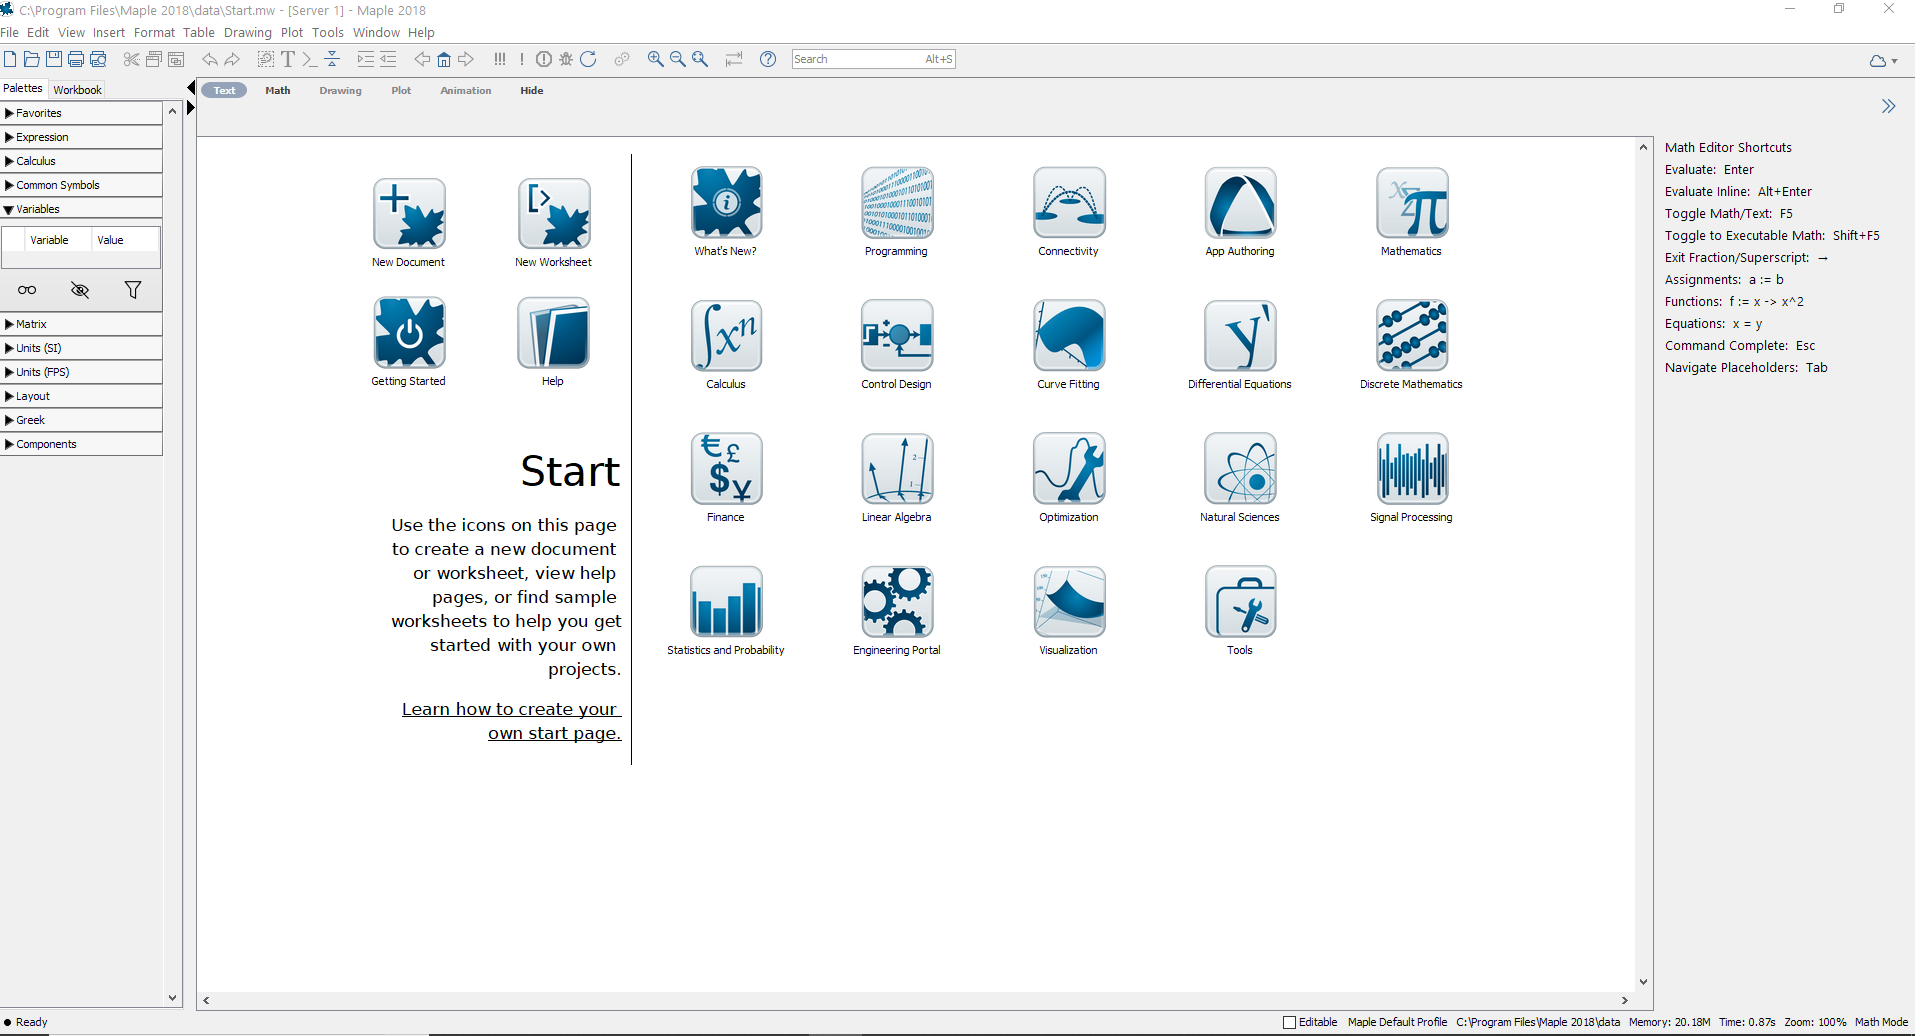
\includegraphics{figs/Maple-Start.png}
\caption{Maple start page screenshot}
\end{figure}

\begin{itemize}
\tightlist
\item
  If you already know what you want to do, then you may open a new document by clicking \texttt{New\ Document} icon in the start document. The following shows what an new (empty document) looks like.
\end{itemize}

\begin{figure}
\centering
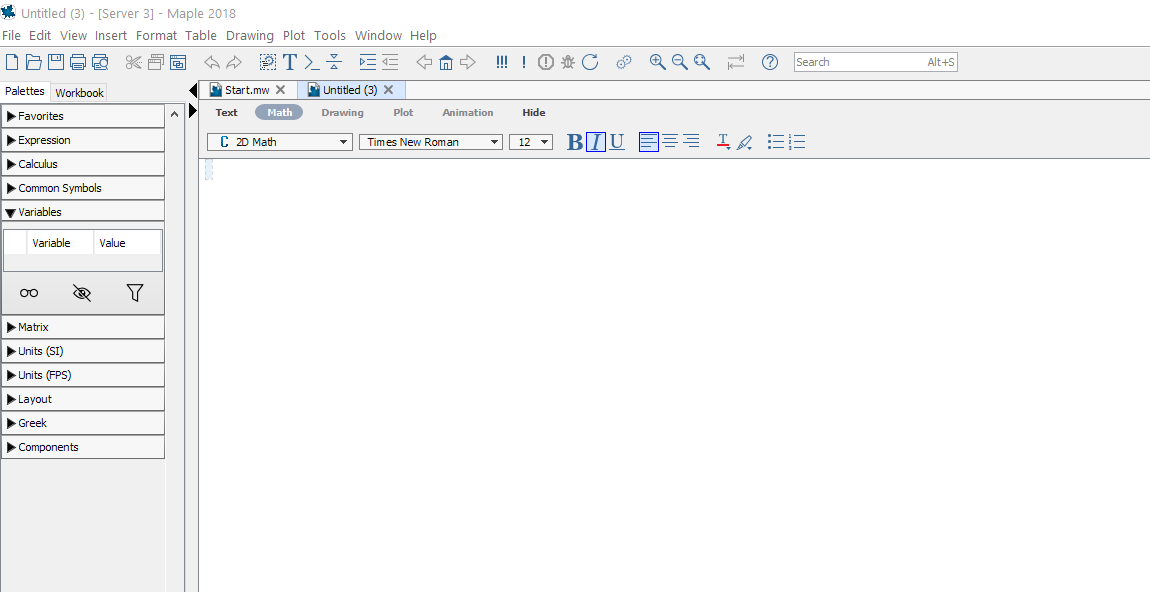
\includegraphics{figs/Maple-New-Doc.png}
\caption{Maple new document page screenshot}
\end{figure}

In this new document you may type in text under \texttt{Text} mode or evaluate a Maple syntax in the \texttt{Math} mode. (See the following picture).

\begin{figure}
\centering
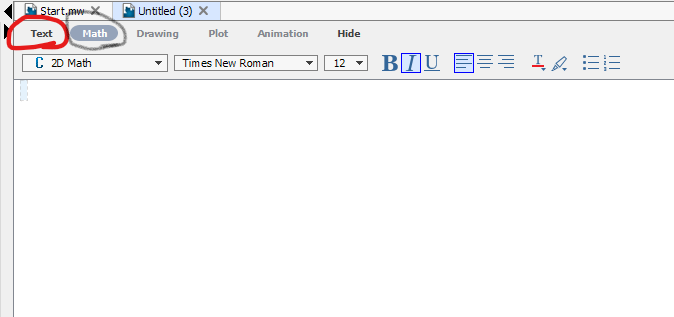
\includegraphics{figs/Text-Math-Mode.png}
\caption{Maple text and Math modes screen shot}
\end{figure}

\begin{itemize}
\item
  If you want to explore some featured sample documents, you may go to \texttt{Start.mw} document and click on different icons to open a new document.

  \begin{itemize}
  \tightlist
  \item
    You may alway reopen the start page by click the home icon to reopen the start page.
  \end{itemize}

  \begin{figure}
  \centering
  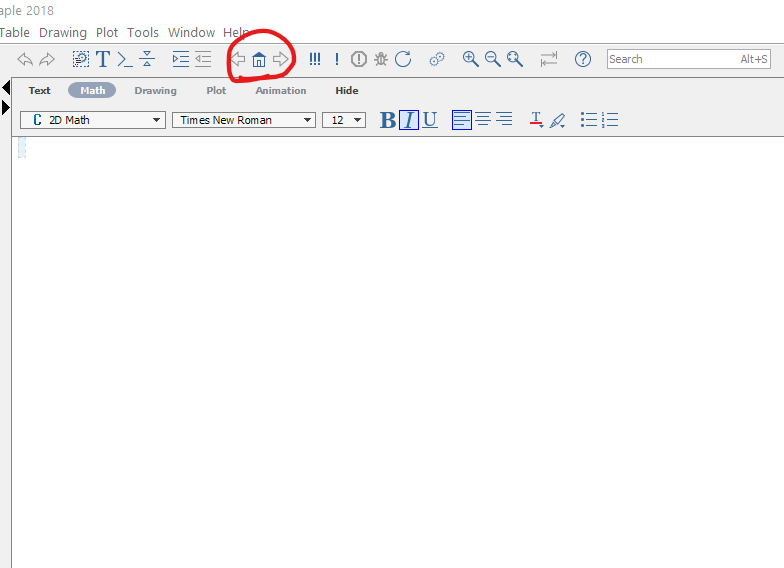
\includegraphics{figs/Home-reopen-start-page.png}
  \caption{Maple reopen start page screenshot}
  \end{figure}
\item
  For Calculus, the most useful document is \texttt{Calculus}.
\end{itemize}

\begin{figure}
\centering
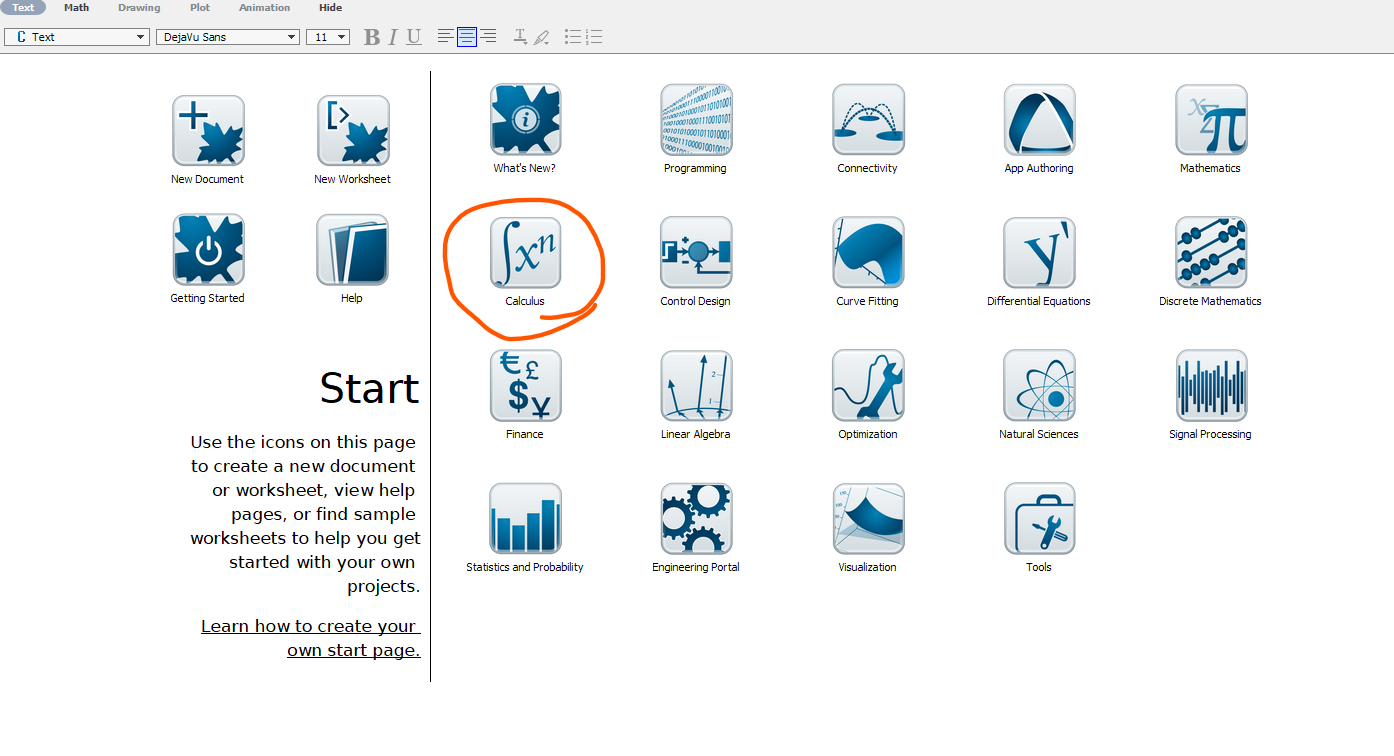
\includegraphics{figs/Start-Page-Calculus.png}
\caption{Maple start page screen shot with Calculus highlighted}
\end{figure}

If you click the \texttt{Calculus} icon on the Start page and click \texttt{OK}, you will see the following document.

\begin{figure}
\centering
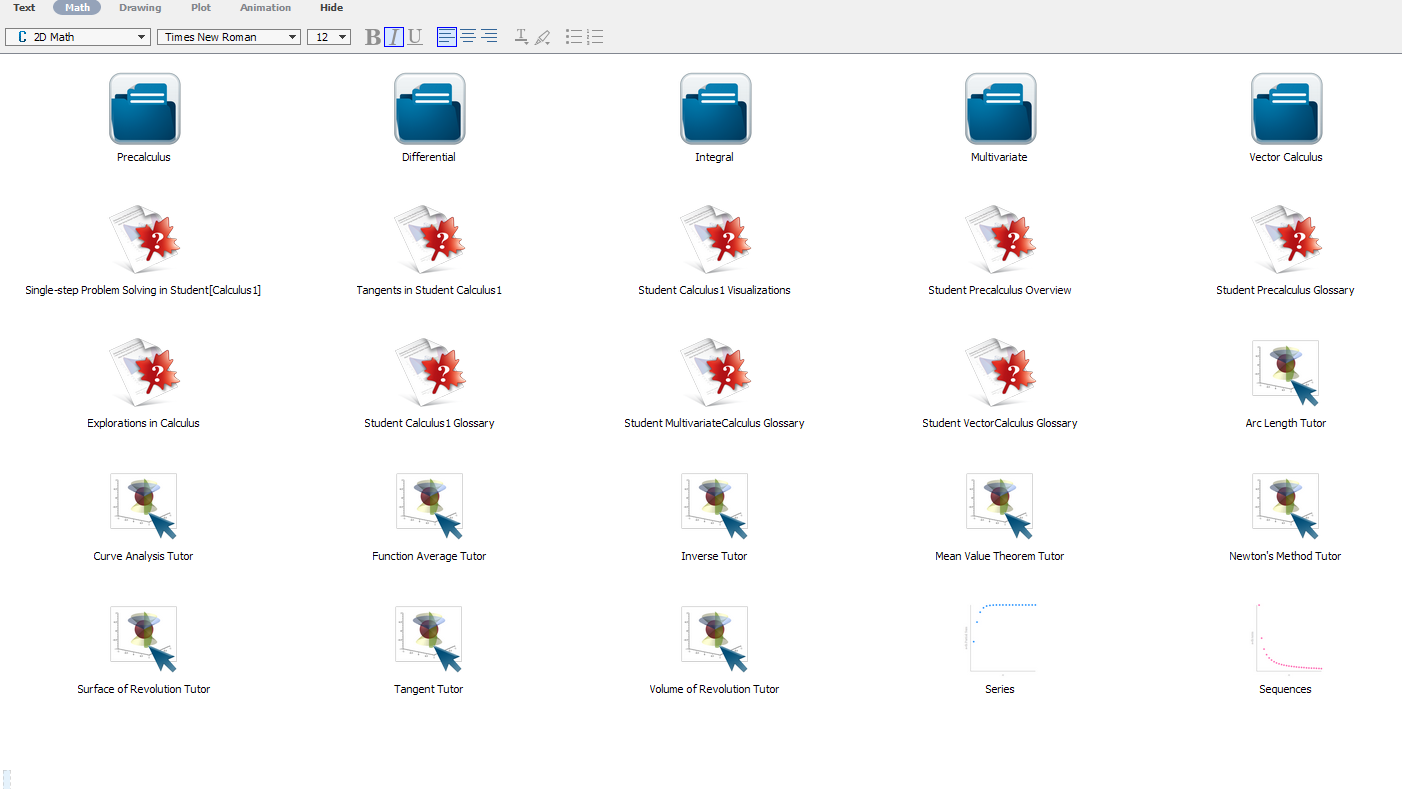
\includegraphics{figs/Calculus-Doc.png}
\caption{Maple Calculus document page screen shot}
\end{figure}

\hypertarget{basic-operators}{%
\section{Basic Operators}\label{basic-operators}}

The first thing to know when learn something new is where and how to get help. In Maple, you may simply type

\begin{verbatim}

?keyword
\end{verbatim}

to open a help page (a new window).

For example, the command \texttt{?operators} will lead you to descriptions of arithmetic operators in Maple.

\begin{longtable}[]{@{}cccccc@{}}
\toprule
& addition & subtraction & multiplication & division & exponentiation\tabularnewline
\midrule
\endhead
Maple Operators & \texttt{+} & \texttt{-} & \texttt{*} & \texttt{/} & \texttt{\^{}}\tabularnewline
In writing & \(x+2\) & \(a-b\) & \(2x\) & \(\dfrac pq\) & \(b^5\)\tabularnewline
In Maple & \texttt{x+2} & \texttt{a-b} & \texttt{2*x} & \texttt{p/q} & \texttt{b\^{}5}\tabularnewline
\bottomrule
\end{longtable}

\hypertarget{how-to-define-a-function}{%
\section{How to define a function}\label{how-to-define-a-function}}

A function is an assignment, for a given input \(x\), we assignment an output \(y\) under a certain rule. Maple take this idea to define functions. The command to define a function has the following form.

\begin{verbatim}

function name:= independent variable -> function rule
\end{verbatim}

Here \texttt{:=} means ``defined/assigned to be'' and \texttt{-\textgreater{}} may be understood as ``plug in''.

\BeginKnitrBlock{example}
\protect\hypertarget{exm:unnamed-chunk-1}{}{\label{exm:unnamed-chunk-1} }
Define the following function in Maple and find the value \(f(0.999)\).

\[
f(x)=\dfrac{x}{x-1}
\]
\EndKnitrBlock{example}

\BeginKnitrBlock{solution}
\iffalse{} {Solution. } \fi{}The function name is \(f\), the independent variable is \(x\) and the function rule is \(\dfrac{x}{x-1}\). So the function can be defined in Maple by the following command.

\begin{verbatim}
f:=x->x/(x-1)
\end{verbatim}

Once the function is define, you may find the function value by the command \texttt{f(0.999)}.
\EndKnitrBlock{solution}

\BeginKnitrBlock{exercise}
\protect\hypertarget{exr:unnamed-chunk-3}{}{\label{exr:unnamed-chunk-3} }
Define the following function in Maple and find the value \(f(2.0001)\).

\[
g(x)=\dfrac{x^3}{(x-2)^2}
\]
\EndKnitrBlock{exercise}

\BeginKnitrBlock{remark}
\iffalse{} {Remark. } \fi{}
The assignment operator \texttt{:=} to the left-hand side the value of the right-hand side. The left-hand side normally is a name and the right-hand side is a value or expression.
\EndKnitrBlock{remark}

\hypertarget{initially-known-mathematical-functions}{%
\section{Initially known mathematical functions}\label{initially-known-mathematical-functions}}

Maple has many predefined functions which can be used to create new functions. To see all initially known mathematical functions in maple, you may use the help command \texttt{?functions} and click the hyperlinked ``initial functions'' in the description shown in the new window.

\begin{figure}
\centering
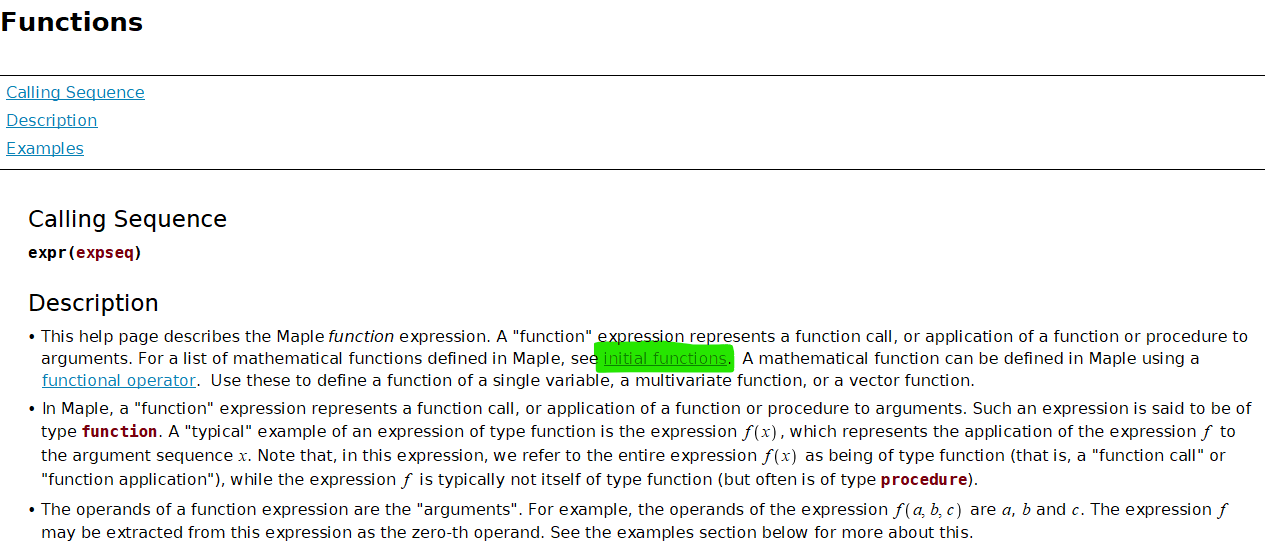
\includegraphics{figs/Initial-Functions.PNG}
\caption{Maple function help page screenshot}
\end{figure}

Some frequently used functions are listed in tables below.

\begin{longtable}[]{@{}ccccc@{}}
\toprule
absolute value & square root & n-th root & natural exponential & logarithmic\tabularnewline
\midrule
\endhead
\texttt{abs()} & \texttt{sqrt()} & \texttt{surd(,n)} & \texttt{exp()} & \texttt{log()},\texttt{log{[}b{]}()}, \texttt{ln()}\tabularnewline
\bottomrule
\end{longtable}

\begin{longtable}[]{@{}cccccc@{}}
\toprule
sine & cosine & tangent & cotangent & secant & cosecant\tabularnewline
\midrule
\endhead
\texttt{sin()} & \texttt{cos()} & \texttt{tan()} & \texttt{cot()} & \texttt{sec()} & \texttt{csc()}\tabularnewline
\bottomrule
\end{longtable}

\begin{longtable}[]{@{}cccccc@{}}
\toprule
\begin{minipage}[b]{0.13\columnwidth}\centering
inverse sine\strut
\end{minipage} & \begin{minipage}[b]{0.13\columnwidth}\centering
inverse cosine\strut
\end{minipage} & \begin{minipage}[b]{0.13\columnwidth}\centering
inverse tangent\strut
\end{minipage} & \begin{minipage}[b]{0.16\columnwidth}\centering
inverse cotangent\strut
\end{minipage} & \begin{minipage}[b]{0.13\columnwidth}\centering
inverse secant\strut
\end{minipage} & \begin{minipage}[b]{0.15\columnwidth}\centering
inverse cosecant\strut
\end{minipage}\tabularnewline
\midrule
\endhead
\begin{minipage}[t]{0.13\columnwidth}\centering
\texttt{arcsin()}\strut
\end{minipage} & \begin{minipage}[t]{0.13\columnwidth}\centering
\texttt{arccos()}\strut
\end{minipage} & \begin{minipage}[t]{0.13\columnwidth}\centering
\texttt{arctan()}\strut
\end{minipage} & \begin{minipage}[t]{0.16\columnwidth}\centering
\texttt{arccot()}\strut
\end{minipage} & \begin{minipage}[t]{0.13\columnwidth}\centering
\texttt{arcsec()}\strut
\end{minipage} & \begin{minipage}[t]{0.15\columnwidth}\centering
\texttt{arccsc()}\strut
\end{minipage}\tabularnewline
\bottomrule
\end{longtable}

Another initially know function that we will use is the piecewise function.

\begin{verbatim}

piecewise(condition1, expression1, condition2, expression2, expression3)
\end{verbatim}

\BeginKnitrBlock{example}
\protect\hypertarget{exm:unnamed-chunk-5}{}{\label{exm:unnamed-chunk-5} }
Define the following function in Maple and evaluate \(pwf(3)\)

\[
pwf(x) =
  \begin{cases}
    \sqrt{\sin(x)} & x<-1\\
    \frac{\sqrt[3]{x}}{|x+2|} & -1\leq x<\pi\\
    \ln(e^x+2) & \text{otherwise}.
  \end{cases}
\]
\EndKnitrBlock{example}

\BeginKnitrBlock{solution}
\iffalse{} {Solution. } \fi{}
The function can be defined by the following command.

\begin{verbatim}
pwf:=x->piecewise(x<-1, sqrt(sin(x)), x>=-1 and x<Pi,
surd(x, 3)/abs(x+2), ln(exp(x)+2))
\end{verbatim}

The value \(pwf(3)\) can be obtained by the command \texttt{pwf(3)}.
\EndKnitrBlock{solution}

\BeginKnitrBlock{exercise}
\protect\hypertarget{exr:piecewise-exer1}{}{\label{exr:piecewise-exer1} }
Define the following function in Maple and evaluate \(q(1)\)

\[
q(x) =
\begin{cases}
  |x-2|/\sqrt{x} & x>\dfrac{pi}{2}\\
  (x-1)\tan(x) & 0\leq x< \dfrac{\pi}{2}\\
  \sqrt[5]{\log_2(1+e^x)} & \text{otherwise}
\end{cases}
\]
\EndKnitrBlock{exercise}

\hypertarget{plot-functions}{%
\section{Plot functions}\label{plot-functions}}

In Maple, you may plot a single variable function easily using the command

\begin{verbatim}

plot(expression, domain, options)
\end{verbatim}

or plot several single variable functions together using

\begin{verbatim}

plot([experssion1, experssion2], domain, options)
\end{verbatim}

In the command, options may be omitted, but the domain must be given.
To see details about available options, you may run the command \texttt{?plot} in Maple.

\BeginKnitrBlock{example}
\protect\hypertarget{exm:unnamed-chunk-7}{}{\label{exm:unnamed-chunk-7} }
Plot the functions \(f(x)=x^2\) in red and \(l(x)=2x+1\) in blue over the domain \([-1, 2]\).
\EndKnitrBlock{example}

\BeginKnitrBlock{solution}
\iffalse{} {Solution. } \fi{}
Here are the command and the output

\begin{verbatim}
plot([x^2, 2*x+1], x=-1..2, color=[red, blue])
\end{verbatim}

\begin{figure}
\centering
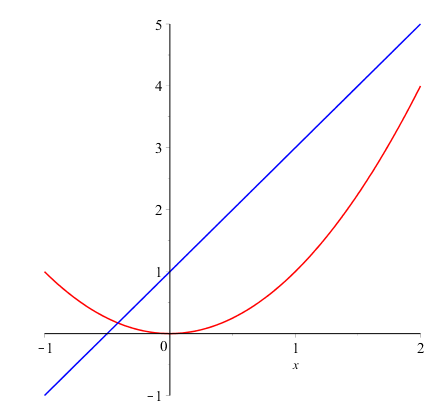
\includegraphics{figs/First-Plot-Example.png}
\caption{Screen shot of the output generated by plotting of two function}
\end{figure}
\EndKnitrBlock{solution}

\BeginKnitrBlock{exercise}
\protect\hypertarget{exr:unnamed-chunk-9}{}{\label{exr:unnamed-chunk-9} }
Plot the piecewise function in Exercise \ref@{piecewise-exer1} over the domain \([-2, 4]\).
\EndKnitrBlock{exercise}

\BeginKnitrBlock{exercise}
\protect\hypertarget{exr:unnamed-chunk-10}{}{\label{exr:unnamed-chunk-10} }
Plot the functions \(f(x)=\ln(x+5)\) and \(g(x)=3\cos(2x+1)+4\) over the domain \([-\pi, \pi]\).
\EndKnitrBlock{exercise}

\hypertarget{part-part-1---calculus-i}{%
\part*{Part 1 - Calculus I}\label{part-part-1---calculus-i}}
\addcontentsline{toc}{part}{Part 1 - Calculus I}

\hypertarget{limits}{%
\chapter{Limits}\label{limits}}

\hypertarget{understand-limits-using-tangent-lines}{%
\section{Understand limits using tangent lines}\label{understand-limits-using-tangent-lines}}

Intuitively, the limit of a function \(f\) at \(x=a\) is a fixed value \(L\) that values of the function \(f(x)\) approach as the values of \(x\) \((\ne a)\) approach \(a\).

The slope of a tangent line to the graph of a functions is a limit of slopes of secant lines. This can be visualized easily using Maple with the support of the package \texttt{Student{[}Calculus1{]}}.

Like predefined functions in Maple, package consists of predefine commands for Maple. The package \texttt{Student} serves for studying Calculus and other subject interactively. The subpackage \texttt{Student{[}Calculus1{]}} focus mainly on Calculus as the name indicated.

As different package has different focus and serves for different purpose, Maple won't load a specific package until you run the command \texttt{with(package\_name)}. For example, the command
\texttt{with(Student{[}Calculus1{]})} will load the subpackage \texttt{Calculus1}.

\BeginKnitrBlock{example}
\protect\hypertarget{exm:unnamed-chunk-11}{}{\label{exm:unnamed-chunk-11} }
Observe how do secant lines of the function \(f(x)=x^3-2\) approach to the tangent line at \(x=1\).
\EndKnitrBlock{example}

\BeginKnitrBlock{solution}
\iffalse{} {Solution. } \fi{}Load the \texttt{Student{[}Calculus1{]}} package using \texttt{with()}.

\begin{verbatim}
with(Student[Calculus1])
\end{verbatim}

Use \texttt{TangentSecantTutor} from the loaded package to observe changes of secant lines.

\begin{verbatim}
TangentSecantTutor(x^3-1, x=1)
\end{verbatim}
\EndKnitrBlock{solution}

\BeginKnitrBlock{exercise}
\protect\hypertarget{exr:unnamed-chunk-13}{}{\label{exr:unnamed-chunk-13} }Explore the package \texttt{Student}, in particular the subpackage \texttt{Student{[}Calculus1{]}}.
You can use the command \texttt{?Student} to get help.

Find the slope of the tangent line to the function \(f(x)=2x^3+\frac1{x^2}\) at \(x=1\) using the \texttt{TangentSecantTutor} command.
\EndKnitrBlock{exercise}

\hypertarget{estimate-limits-numerically-or-graphically}{%
\section{Estimate limits numerically or graphically}\label{estimate-limits-numerically-or-graphically}}

To estimate a limit \(\lim\limits_{x\to a}f(x)\) numerically, one may pick some values close to \(a\) and evaluate the function. In Maple, the calculation can be done by using the repetition statement \texttt{for\ counter\ in\ array\ do\ statement\ end\ to;}.

\BeginKnitrBlock{example}
\protect\hypertarget{exm:unnamed-chunk-14}{}{\label{exm:unnamed-chunk-14} }Estimate the limit \(\lim\limits_{x\to 0}\frac{\sin x}{x}\) by approximations.
\EndKnitrBlock{example}

\BeginKnitrBlock{solution}
\iffalse{} {Solution. } \fi{}First, we pick some values close to 0, for example -0.99, -0.999, -0.9999, 0.01, 0.001, 0.0001 and assign them to an expression.

\begin{verbatim}
sq:=[-0.99, -0.999, -0.9999, 0.0001, 0.001, 0.01]
\end{verbatim}

Now we find the function values using two new commands instead of defining the function a priori.

\begin{verbatim}
for t in sq do evalf(subs(x=t, sin(x)/x)) end do;
\end{verbatim}
\EndKnitrBlock{solution}

Graphs provide visual intuition which helps understand and solve problems. Recall, the command \texttt{plot(expression,\ domain,\ option)} produces a graph of the function defined by the expression over your choice of domain.

\BeginKnitrBlock{example}
\protect\hypertarget{exm:unnamed-chunk-16}{}{\label{exm:unnamed-chunk-16} }
Determine whether the limit \(\lim\limits_{x\to 0}\frac{1}{1- \cos x}\) exists.
\EndKnitrBlock{example}

\BeginKnitrBlock{solution}
\iffalse{} {Solution. } \fi{}
Apply the \texttt{plot} function to the expression over the domain \((-0.5, 0.5)\).

\begin{verbatim}
plot(1/(1-cos(x)), x=-0.5..0.5)
\end{verbatim}

The graph shows that the function \(y=\frac{1}{1- \cos x}\) goes to \(\infty\) when \(x\) approaches \(0\). So the limit is an infinite limit.
\EndKnitrBlock{solution}

\BeginKnitrBlock{exercise}
\protect\hypertarget{exr:unnamed-chunk-18}{}{\label{exr:unnamed-chunk-18} }
Estimate the limit \(\lim\limits_{t \to 0}\frac{1-\cos x}{x}\) numerically.
\EndKnitrBlock{exercise}

\BeginKnitrBlock{exercise}
\protect\hypertarget{exr:unnamed-chunk-19}{}{\label{exr:unnamed-chunk-19} }
Determine whether the limit \(\lim\limits_{x \to 1}\frac{\sin x}{|x-1|}\) exists using the graph.
\EndKnitrBlock{exercise}

\hypertarget{evaluate-limits}{%
\section{Evaluate limits}\label{evaluate-limits}}

Maple provides the following command to evaluate a limit

\begin{verbatim}

limit(function, position, direction)
\end{verbatim}

The direction may be omitted when evaluating a two-side limit.

\BeginKnitrBlock{example}
\protect\hypertarget{exm:unnamed-chunk-20}{}{\label{exm:unnamed-chunk-20} }
Determine whether the limit \(\lim\limits_{x\to 0}\frac{|x|}{x}\) exists.
\EndKnitrBlock{example}

\BeginKnitrBlock{solution}
\iffalse{} {Solution. } \fi{}
You may find the left and right limits using the following commands.

\begin{verbatim}
limit(abs(x)/x, x=0, left)
limit(abs(x)/x, x=0, right)
\end{verbatim}

It turns out that \(\lim\limits_{x\to 0}\frac{|x|}{x}\) does not exist because the left limit and the right limit are different.
\EndKnitrBlock{solution}

\BeginKnitrBlock{example}
\protect\hypertarget{exm:unnamed-chunk-22}{}{\label{exm:unnamed-chunk-22} }
Evaluate the limit \(\lim\limits_{h\to 0}\dfrac{f(x+h)-f(x)}{h}\), where \(f(x)=\dfrac{1}{x}\).
\EndKnitrBlock{example}

\BeginKnitrBlock{solution}
\iffalse{} {Solution. } \fi{}
The limit can be obtained using the following command.

\begin{verbatim}
limit((1/(x+h)-1/x)/h, x=0)
\end{verbatim}
\EndKnitrBlock{solution}

\BeginKnitrBlock{exercise}
\protect\hypertarget{exr:unnamed-chunk-24}{}{\label{exr:unnamed-chunk-24} }
Determine whether the limit \(\lim\limits_{x\to 1/2}\dfrac{2x-1}{|2x^3-x^2|}\) exists.
\EndKnitrBlock{exercise}

\BeginKnitrBlock{exercise}
\protect\hypertarget{exr:unnamed-chunk-25}{}{\label{exr:unnamed-chunk-25} }
Evaluate the limit \(\lim\limits_{t\to 0}\dfrac{\sqrt{x+t}-\sqrt{x}}{t}\).
\EndKnitrBlock{exercise}

\hypertarget{learn-limit-laws-using-limittutor}{%
\section{\texorpdfstring{Learn limit laws using \texttt{LimitTutor}}{Learn limit laws using LimitTutor}}\label{learn-limit-laws-using-limittutor}}

Suppose the limits of two functions \(f\) and \(g\) at the same point \(x=a\) exist (equal finite numbers). Then the limit operation commutes with addition/subtraction, multiplication/division and power.

In Maple, you may use the command \texttt{LimitTutor(function,\ position,\ direction)}, which is again supported by the subpackage \texttt{Student{[}Calculus1{]}}, to learn how to evaluate a limit using limit laws and theorems.

\BeginKnitrBlock{example}
\protect\hypertarget{exm:unnamed-chunk-26}{}{\label{exm:unnamed-chunk-26} }
Evaluate \(\lim\limits_{x\to 0}\dfrac{1-\cos x}{x}\).
\EndKnitrBlock{example}

\BeginKnitrBlock{solution}
\iffalse{} {Solution. } \fi{}
Load the subpackage \texttt{Student{[}Calculus1{]}} if it was not loaded.

\begin{verbatim}
with(Student[Calculus1])
\end{verbatim}

Use the following command to learn how to evaluate the limit.

\begin{verbatim}
LimitTutor(2-x^3, x=2,'right')
\end{verbatim}

You will see an interactive windows pop out. You can choose the see the procedure step-by-step.
\EndKnitrBlock{solution}

\BeginKnitrBlock{exercise}
\protect\hypertarget{exr:unnamed-chunk-28}{}{\label{exr:unnamed-chunk-28} }
Evaluate \(\lim\limits_{x\to 0}\dfrac{(x+2)(\cos x-1)}{x^2-x}\) using \texttt{LimitTutor}.
\EndKnitrBlock{exercise}

\hypertarget{squeeze-theorem}{%
\section{Squeeze Theorem}\label{squeeze-theorem}}

Comparison is a very useful tool in problem solving. Squeeze theorem is such an example

\BeginKnitrBlock{theorem}[Squeeze Theorem]
\protect\hypertarget{thm:unnamed-chunk-29}{}{\label{thm:unnamed-chunk-29} \iffalse (Squeeze Theorem) \fi{} }
Suppose that
\[
f(x)\leq g(x)\leq h(x)
\]
and
\[
\lim\limits_{x\to c}f(x)=L=\lim\limits_{x\to c}h(x).
\]
Then
\[
\lim\limits_{x\to c}g(x)=L.
\]
\EndKnitrBlock{theorem}

Let's use Maple to understand the statement.

\BeginKnitrBlock{example}
\protect\hypertarget{exm:unnamed-chunk-30}{}{\label{exm:unnamed-chunk-30} }
Graph the functions \(f(x)=-x\), \(g(x)=x\cos\frac1x\) and \(h(x)=x\) in the same coordinate system. What's the limit of \(g(x)\) as \(x\) approaches \(0\).
\EndKnitrBlock{example}

\BeginKnitrBlock{solution}
\iffalse{} {Solution. } \fi{}
We use the \texttt{plot()} command to graph the functions together.

\begin{verbatim}
plot([-x, x*cos(1/x), x], x=-1..1, discont, color=[red, blue, red])
\end{verbatim}

\begin{figure}
\centering
\includegraphics{figs/squeeze.png}
\caption{Squeeze Theorem demonstration}
\end{figure}

From the graph, we see that the \(\lim\limits_{x\to c}f(x)=0\) as it is squeezed by two limits which are both \(0\).
\EndKnitrBlock{solution}

\BeginKnitrBlock{exercise}
\protect\hypertarget{exr:unnamed-chunk-32}{}{\label{exr:unnamed-chunk-32} }
Graph the functions \(f(x)=-x\), \(g(x)=x\sin\frac1x\) and \(h(x)=x\) in the same coordinate system. What's the limit of \(g(x)\) as \(x\) approaches \(0\).
\EndKnitrBlock{exercise}

\hypertarget{continuity}{%
\section{Continuity}\label{continuity}}

A function \(f\) is continuous at \(x=a\) if \(f(a)\) is defined and \(\lim\limits_{x\to a}f(x)=f(a)\). Intuitively, a function is continuous if the graph has no hole or jump.

\BeginKnitrBlock{example}
\protect\hypertarget{exm:unnamed-chunk-33}{}{\label{exm:unnamed-chunk-33} }
Use graph to determine if the function
\[
f(x)=
\begin{cases}
    x & x\le -1 \\
    1/(x-1) & -1<x<1\\
    3-x & 1<x\le 2\\
    \sin(x - 2) + 1 & x>2\\
    -2 & x=2
\end{cases}
\]
is continuous over \((-\infty, \infty)\). Find the discontinuities and verify them using the definition and properties of continuity.
\EndKnitrBlock{example}

\BeginKnitrBlock{solution}
\iffalse{} {Solution. } \fi{}
First we define the function.

\begin{verbatim}
f := x -> piecewise(x <= -1, x, -1 < x and x < 1, 1/(x - 1), 1 <= x and x < 2, 3 - x, 2 < x, sin(x - 2) + 1, -2)
\end{verbatim}

We first check visually whether the graph has holes or jumps.

\begin{verbatim}
plot(f(x), discont=[showremovable], x=-5..5, smartview=true)
\end{verbatim}

In the above command, the option \texttt{discont\ =\ {[}showremovable{]}} is used to show removable discontinuities.

\begin{figure}
\centering
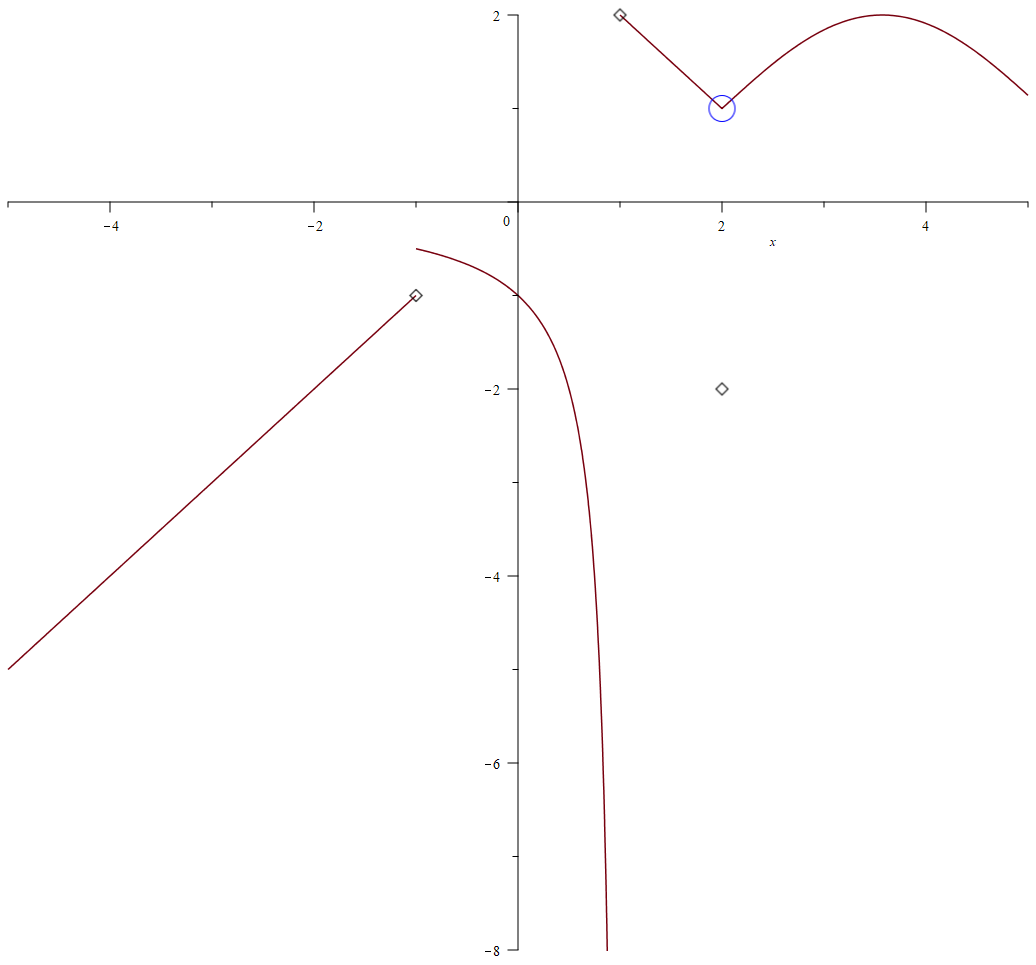
\includegraphics{figs/Discontinuities.png}
\caption{An example shows three types of discontinuities}
\end{figure}

From the graph, we can tell that the function has discontinuities which can also be found using Maple.

\begin{verbatim}
discont(f(x), x)
\end{verbatim}

Maple gives three discontinuities \(\{-1, 1, 2\}\).

Let's first find limits at all three values.

\begin{verbatim}
discontset:=[-1, 1, 2]
for a in discontset do limit(f(x), x=a) end do
\end{verbatim}

You will find that limits do not exist at \(-1\) and \(1\). The limit at \(2\) is \(1\).
However, \(g(2)=-2\). So \(f\) has three discontinuities at \(x=-1\), \(x=1\) and \(x=2\).
\EndKnitrBlock{solution}

\BeginKnitrBlock{exercise}
\protect\hypertarget{exr:unnamed-chunk-35}{}{\label{exr:unnamed-chunk-35} }Determine if the function
\[
f(x)=
\begin{cases}
    -x^2+2 & x\le 1 \\
    \tan x& 1<x<\pi/2\\
    2\cos x-1 & \text{otherwise}
\end{cases}
\]
is continuous over \((-\infty, \infty)\).
Find all discontinuities if they exist and verify them using the definition.
\EndKnitrBlock{exercise}

\hypertarget{continuity-and-limit-of-a-composite-function}{%
\section{Continuity and Limit of a Composite Function}\label{continuity-and-limit-of-a-composite-function}}

Continuous functions behave under composition. The composition of continuous functions is still continuous over its domain. More generally,

\BeginKnitrBlock{theorem}
\protect\hypertarget{thm:unnamed-chunk-36}{}{\label{thm:unnamed-chunk-36} }Let \(f\) be a function continuous at \(x=L\). Suppose that \(\lim\limits_{x\to c}g(x)=L\). Then
\[
\lim{x\to c}f(g(x))=f(L).
\]
\EndKnitrBlock{theorem}

In general, the limit does not commute with composition.

\BeginKnitrBlock{example}
\protect\hypertarget{exm:unnamed-chunk-37}{}{\label{exm:unnamed-chunk-37} }
Let
\[
f(x)=x^3\quad \text{and}\quad
g(x)=
\begin{cases}
1 & x=0\\
2x-1 & \text{otherwise}
\end{cases}
\]

Verify that
\[
\lim_{x\to 0}f(g(x))=f(\lim_{x\to 0}g(x)).
\]

Is is true that
\[
\lim_{x\to 0}g(f(x))=g(\lim_{x\to 0}f(x))?
\]
\EndKnitrBlock{example}

\BeginKnitrBlock{solution}
\iffalse{} {Solution. } \fi{}We first define \(f\) and \(g\) in Maple

\begin{verbatim}
f:=x->x^2
g:=x->piecewise(x=0, 0, x+2)
\end{verbatim}

Evaluate limits for \(f\circ g\).

\begin{verbatim}
limit(f(g(x)), x=0)
f(limit(g(x), x=0))
\end{verbatim}

The results verify that the limit commutes with composition if the outside function is continuous.

Evaluate limits for \(g\circ f\)

\begin{verbatim}
limit(f(g(x)), x=0)
f(limit(g(x), x=0))
\end{verbatim}

The results show that the limit may not commute with composition if the outside function is not continuous.
\EndKnitrBlock{solution}

\BeginKnitrBlock{exercise}
\protect\hypertarget{exr:unnamed-chunk-39}{}{\label{exr:unnamed-chunk-39} }
Find three functions \(f\), \(g\), \(h\) and a value \(c\) such that \(f(g(x))\) is continuous,
\[
\lim\limits_{x\to c}f(h(x))=f(\lim\limits_{x\to c}h(x))
\]
and
\[
\lim\limits_{x\to c}h(g(x))\neq h(\lim\limits_{x\to c}g(x)).
\]
\EndKnitrBlock{exercise}

\hypertarget{intermediate-value-theorem}{%
\section{Intermediate Value Theorem}\label{intermediate-value-theorem}}

A very important result about continuity is the intermediate value theorem (IVT for short).

\BeginKnitrBlock{theorem}[Intermediate Value Theorem]
\protect\hypertarget{thm:unnamed-chunk-40}{}{\label{thm:unnamed-chunk-40} \iffalse (Intermediate Value Theorem) \fi{} }Let \(f\) be a function continuous over the interval \([a, b]\). Suppose that \(f(a)\neq f(b)\) and \(N\) is a number between \(f(a)\) and \(f(b)\). Then there exists a number \(c\in (a, b)\) such that \(f(c)=N\).

In particular, if \(f(a)f(b)<0\) then there exists a number \(c\) such that \(f(c)=0\).
\EndKnitrBlock{theorem}

\BeginKnitrBlock{example}
\protect\hypertarget{exm:unnamed-chunk-41}{}{\label{exm:unnamed-chunk-41} }
Determine whether the equation
\[
\sin^2x+2x-1=0
\]
has the solution in \((-1, 1)\). Estimate the solution if it exists.
\EndKnitrBlock{example}

\BeginKnitrBlock{solution}
\iffalse{} {Solution. } \fi{}
We first use the left hand side of the equation to define a function \(eql\).

eql:=x-\textgreater sin(x)\^{}2 + 2*x - 1

Now lets verify that \(eql\) is continuous over \([-1,1]\) using the command \texttt{iscont()}.

\begin{verbatim}
iscont(eql(x), x=-1..1)
\end{verbatim}

The result is \texttt{True}. We may apply the IVT. Let's check if the value \(eql(-1)\cdot eql(1)<0\).

\begin{verbatim}
evalf(eql(-1)*eql(1))
\end{verbatim}

Here \texttt{evalf()} convert the symbolic answer to the (approximate) numerical value.

Since the product is negative, applying the IVT, we know there exists a solution between \((-1, 1)\).

This can also be seen from the graph using the command.

\begin{verbatim}
plot(eql(x), x=-1..1)
\end{verbatim}

To estimate the solution, you may use the Maple command

\begin{verbatim}
evalf(solve(eql(x) = 0, x))
\end{verbatim}

or you may repeatedly apply IVT to find an approximate solution.

\begin{verbatim}
m:=10;
a:=-1;
b:=1;
for n from 1 to m do
    c[n] := (a + b)/2;
    if evalf(eql(c[n])*eql(a)) < 0 then
        b := c[n];
    else
        a := c[n];
    end if;
    evalf(eql(c[n]));
end do;
\end{verbatim}
\EndKnitrBlock{solution}

\BeginKnitrBlock{exercise}
\protect\hypertarget{exr:unnamed-chunk-43}{}{\label{exr:unnamed-chunk-43} }
Find an integer \(k\) such that the equation
\[
\cos^2x + 3x - 2=0
\]
has a solution in \((k, k+1)\). Estimate the solution.
\EndKnitrBlock{exercise}

\hypertarget{derivatives}{%
\chapter{Derivatives}\label{derivatives}}

\hypertarget{derivative-functions}{%
\section{Derivative Functions}\label{derivative-functions}}

What makes derivative so important in modern mathematics is the ideal of linearly approximating curves using tangent lines. Geometrically, the derivative of a function \(f\) at a point \(x=a\) is the slope of the line tangent to \(f\) at \(x=a\). Using limits (if it exists), the derivative is defined as
\[
f'(a):=\lim\limits_{x\to a}\frac{f(x)-f(a)}{x-a}.
\]

Consider \(a\) as a variable, we may define a function called the derivative function. In terms of limits, the derivative function of a function \(f\), denoted by \(f'\) is given by
\[
f'(x)=\lim\limits_{h\to 0}\frac{f(x+h)-f(x)}{h}.
\]

Using limit laws, we can show that differentiable functions are continuous.

Geometrically, the graph of differentiable function locally is flat without any hole or jump.

All \href{https://en.wikipedia.org/wiki/Elementary_function}{elementary functions} are differentiable over their domain. But there are also many functions which are not differential everywhere in their domain.

\BeginKnitrBlock{example}
\protect\hypertarget{exm:unnamed-chunk-44}{}{\label{exm:unnamed-chunk-44} }
Use the graph of the function \(f(x)=|x-1|\) to identify a \(x\) value where \(f\) is not differential. Verify your finding using the definition of differentiability.
\EndKnitrBlock{example}

\BeginKnitrBlock{solution}
\iffalse{} {Solution. } \fi{}
First plot the function.

\begin{verbatim}
f:= x-> abs(x)

plot(f(x), x=-2..2)
\end{verbatim}

You will see the function is not flat near \(x=1\). To verify that, we calculate the limit of the difference quotient for all \(x\) and then evaluate the resulting function at \(x=1\).

\begin{verbatim}
diffquot:=(f(x+h)-f(x))/h

derlimit:= limit(diffquot, h=0)

evalf(subs(x=1, derlimit))
\end{verbatim}
\EndKnitrBlock{solution}

\BeginKnitrBlock{exercise}
\protect\hypertarget{exr:unnamed-chunk-46}{}{\label{exr:unnamed-chunk-46} }
Determine whether the function
\[
f(x)=\begin{cases}
x\sin\left(\frac1x\right) & x\neq 0\\
0 & x=0
\end{cases}
\]
is differential at \(x=0\) using the definition of the differentiability.
\EndKnitrBlock{exercise}

\BeginKnitrBlock{exercise}
\protect\hypertarget{exr:unnamed-chunk-47}{}{\label{exr:unnamed-chunk-47} }
Determine whether the function
\[
f(x)=\begin{cases}
x^2\cos\left(\frac1x\right) & x\neq 0\\
0 & x=0
\end{cases}
\]
is differential at \(x=0\) using the definition of the differentiability.
\EndKnitrBlock{exercise}

\BeginKnitrBlock{exercise}
\protect\hypertarget{exr:unnamed-chunk-48}{}{\label{exr:unnamed-chunk-48} }
Using the definition to find the derivative for \(y=\sin x\).
\EndKnitrBlock{exercise}

\hypertarget{calculating-derivatives}{%
\section{Calculating Derivatives}\label{calculating-derivatives}}

Calculating a derivative in Maple is as easy as calculating a limit. The command for differentiation is \texttt{diff(function,\ variable)}. For higher derivatives, you may simply repeat the variable or use \texttt{{[}variable\$n{]}} to indicate the \(n\) times differentiation.

\BeginKnitrBlock{example}
\protect\hypertarget{exm:unnamed-chunk-49}{}{\label{exm:unnamed-chunk-49} }
Calculate the first derivative and the second derivative for the function
\[
f(x)=\frac{2}{\sqrt{2\sin^2 x + 1}}.
\]
\EndKnitrBlock{example}

\BeginKnitrBlock{solution}
\iffalse{} {Solution. } \fi{}
First represent the function rule simply by \texttt{f}.

\begin{verbatim}
f:=2/(sqrt(2*(sin(x))^2+1))
\end{verbatim}

Calculate the first derivative and denote the derivative by \texttt{f1}.

\begin{verbatim}
f1:=diff(f, x);
\end{verbatim}

Calculate the second derivative and denote the derivative by \texttt{f2}. You may use one of the following three commands.

\begin{verbatim}
f2:=diff(f1, x)
f2:=diff(f, x, x)
f2:=diff(f, [x$2])
\end{verbatim}
\EndKnitrBlock{solution}

Maple also has a tutoring command for differentiation: \texttt{DiffTutor(function,\ variable)} which is again supported by the subpackage \texttt{Student{[}Calculus1{]}}. However, \texttt{DiffTutor} only works for the first derivative.

\BeginKnitrBlock{example}
\protect\hypertarget{exm:unnamed-chunk-51}{}{\label{exm:unnamed-chunk-51} }
Calculate the derivative for \(g(x)=\frac{x^2-2x-x^{-3}}{\sqrt{x}}\) by hand and compare your calculation the the result given by \texttt{DiffTutor}.
\EndKnitrBlock{example}

\BeginKnitrBlock{solution}
\iffalse{} {Solution. } \fi{}
By hand, we may simplify the expression using rational exponents first and then apply derivative rules.
\[
g'(x)=(x^{\frac32}-2x^{\frac12}-x^{-\frac72})'=\frac32\sqrt{x}-\frac{1}{\sqrt{x}}+\frac{7}{2x^4\sqrt{x}}=\frac{3x^5-2x^4+7}{2x^4\sqrt{x}}.
\]

To see the result from \texttt{DiffTutor}, we use the following command. Remember to load the \texttt{Student{[}Calculus1{]}} first.

\begin{verbatim}
with(Student[Calculus1])
DiffTutor((x^2-2*x-x^(-3))/sqrt(x), x)
\end{verbatim}

Here is how does the output look like

\begin{figure}
\centering
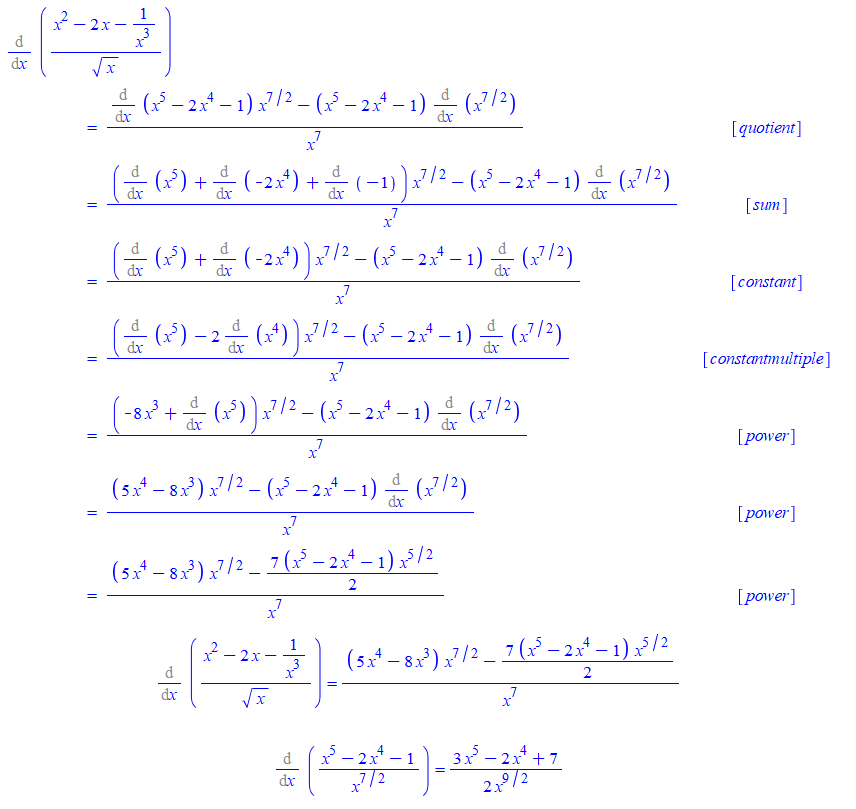
\includegraphics{figs/DiffTutor-Example.png}
\caption{The derivative of a function obtained by the DiffTutor command}
\end{figure}
\EndKnitrBlock{solution}

\BeginKnitrBlock{exercise}
\protect\hypertarget{exr:unnamed-chunk-53}{}{\label{exr:unnamed-chunk-53} }
Calculate the first derivative for the function \(y=2x^{-1}-3\sqrt{x}\) by hand and by Maple. Compare two results. Are they different? If so, can you explain the difference?
\EndKnitrBlock{exercise}

\BeginKnitrBlock{exercise}
\protect\hypertarget{exr:unnamed-chunk-54}{}{\label{exr:unnamed-chunk-54} }
Calculate the first derivative for the function \(y=x\sin^{-1}(x)\) by hand and by Maple. Compare two results. Are they different? If so, can you explain the difference?
\EndKnitrBlock{exercise}

\BeginKnitrBlock{exercise}
\protect\hypertarget{exr:unnamed-chunk-55}{}{\label{exr:unnamed-chunk-55} }
Calculate the first derivative for the function \(y=\frac{\cos(x)+\sin x}{x}\) by hand and by Maple. Compare two results. Are they different? If so, can you explain the difference?
\EndKnitrBlock{exercise}

\BeginKnitrBlock{exercise}
\protect\hypertarget{exr:unnamed-chunk-56}{}{\label{exr:unnamed-chunk-56} }
Calculate the \(3\)-th derivative for the function \(y=\sin x\cos x\) by hand and by Maple. Can you find a formula for the \(n\)-th derivative of the function?
\EndKnitrBlock{exercise}

\hypertarget{chain-rule}{%
\section{Chain Rule}\label{chain-rule}}

Let \(f(x)\) and \(g(x)\) be two differentiable functions. Then the derivative of the composite function \(f(g(x))\) can be calculated using the following formula
\[
(f(g(x)))'=f'(g(x))g'(x).
\]
Why there is an extra factor \(g'(x)\)? This is mainly because \(g(x+h)\approx g(x)+g'(x)h\).

Now let's use Maple to understand the chain rule. In Maple, the symbol for composition is \texttt{@}, that is, in Maple the composition \(f\circ g\) is given by \texttt{f@g}.

Since we will evaluate derivative functions, in addition to the command \texttt{diff(expression,\ variable)}, we will also use \texttt{D(function)(variable)} to find the derivative function. One major difference between those two commands is that \texttt{D} is designed to differentiate functions, whereas \texttt{diff} is for differentiating expressions.

\begin{figure}
\centering
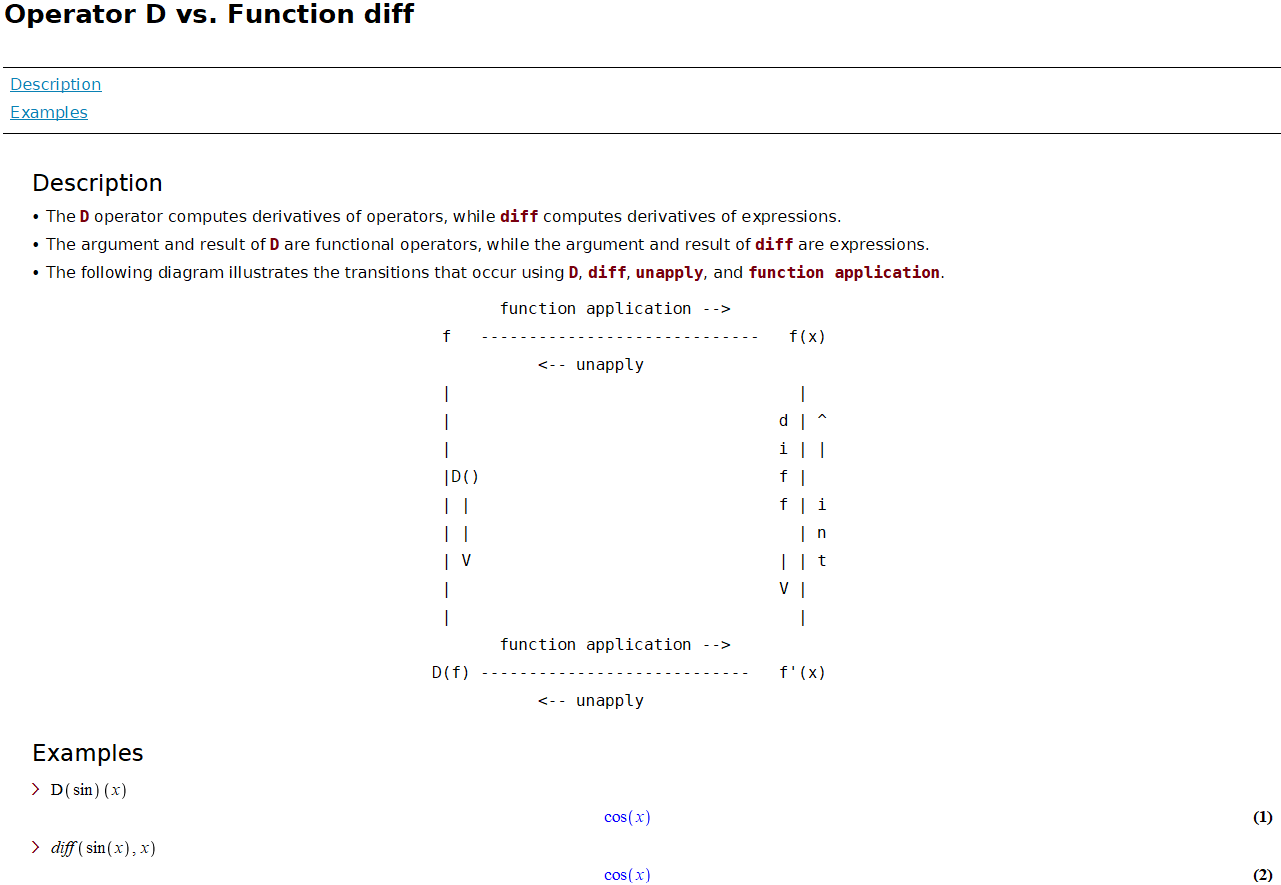
\includegraphics{figs/D_vs_diff.png}
\caption{A screen shot from Maple shows a comparison between the commands D and diff}
\end{figure}

\BeginKnitrBlock{example}
\protect\hypertarget{exm:unnamed-chunk-57}{}{\label{exm:unnamed-chunk-57} }
Let \(f(x)=\sin x\), \(g(x)=2x\) and \(F(x)=2\sin x\cos x\). Find \(f'(g(x))\), \((fg)'(x)\), \((f\circ g)'(x)\) and \(F'(x)\)?
Compare the derivatives and draw a conclusion.
\EndKnitrBlock{example}

\BeginKnitrBlock{solution}
\iffalse{} {Solution. } \fi{}
We first define the functions.

\begin{verbatim}
f:=x->sin(x);
g:=x->2*x;
F:=x->2*sin(x)*cos(x);
\end{verbatim}

Find the derivative functions

\begin{verbatim}
Der_f_g:=D(f)(g(x)); # f'(g(x))
Der_fg:=diff(f(x)g(x), x); # (fg)'(x)
Der_fog:=D(f@g)(x); # (fog)'(x)
Der_F:=D(F)(x); # F'(x)
\end{verbatim}

To compare the derivatives, we use the command \texttt{expand} and \texttt{simplify} to rewrite the expressions.

\begin{verbatim}
simplify(expand(Der_f_g));
simplify(expand(Der_fg));
simplify(expand(Der_fog));
simplify(expand(Der_F));
\end{verbatim}

From the outputs, we see that \((f\circ g)'(x)=F'(x)\). Why they are the same? This is because \(\sin(2x)=2\sin x\cos x\)!.

\begin{figure}
\centering
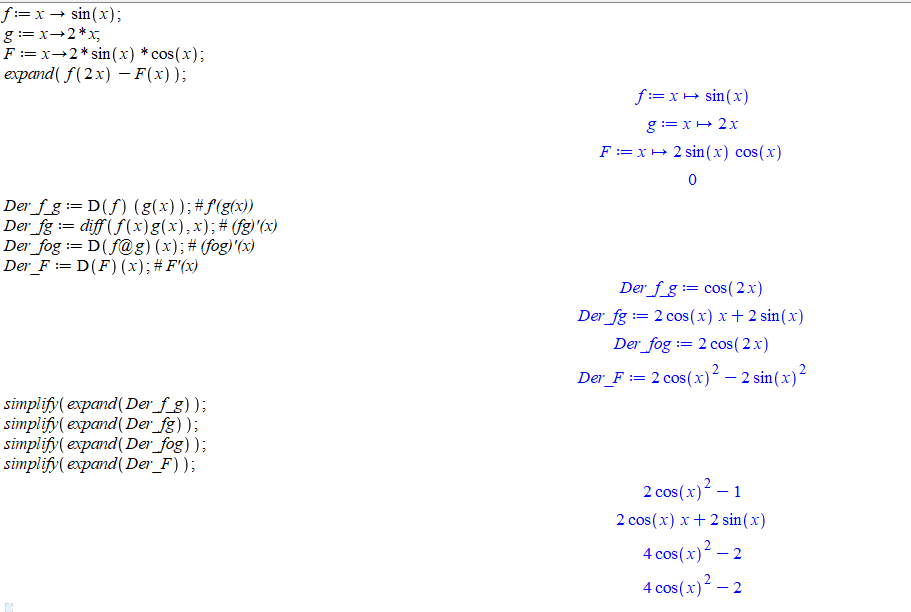
\includegraphics{figs/chain_rule.png}
\caption{An example about the chain rule solved using Maple}
\end{figure}
\EndKnitrBlock{solution}

\BeginKnitrBlock{remark}
\iffalse{} {Remark. } \fi{}
You may also use \texttt{D(unapply(f(x)*g(x),\ x))(x)} to calculate the derivative of the product function \((fg)(x)=f(x)g(x)\).
\EndKnitrBlock{remark}

The chain rule is almost unavoidable in calculation of derivatives. Sometimes, using chain rule will simplify the calculation.

\BeginKnitrBlock{example}
\protect\hypertarget{exm:unnamed-chunk-60}{}{\label{exm:unnamed-chunk-60} }
Consider the function \(f(x)=\frac{1}{\sin x+\cos x}\).

\begin{enumerate}
\def\labelenumi{\arabic{enumi}.}
\tightlist
\item
  Find the derivative function \(f'(x)\) using \texttt{DiffTutor}. Which rule of derivative was applied first?
\item
  Find the point where the tangent line of \(f\) is horizontal over the domain \((-\frac{\pi}{2}, \frac{\pi}{2})\).
\item
  Find an equation of the tangent line at \((0, 1)\).
\item
  Plot the tangent line and the function together over the domain \((-\frac12, \frac12)\).
\end{enumerate}
\EndKnitrBlock{example}

\BeginKnitrBlock{solution}
\iffalse{} {Solution. } \fi{}
You may use quotient rule to find the derivative. However, the chain rule may be a better choice because \(\frac{1}{\sin x+\cos x}=(\sin x+\cos x)^{-1}\). Let's try \texttt{DiffTutor}.

\begin{verbatim}
restart; # Use `restart` to clear the internal memory.
with(Student[Calculus1]);
f:=1/(sin(x)+cos(x));
DiffTutor(f, x);
\end{verbatim}

You see that the chain rule was applied first.

\begin{figure}
\centering
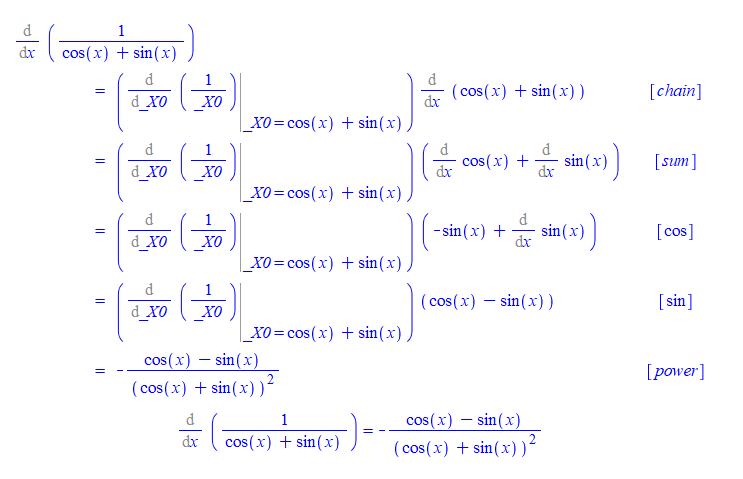
\includegraphics{figs/DiffTutor-Chain-Rule-Example.png}
\caption{A example that chain rule was applied first by DiffTutor}
\end{figure}

To find the points where the tangent line is horizontal, we need to solve the equation \(f'(x)=0\).

\begin{verbatim}
solve(diff(f, x)=0)
\end{verbatim}

To find the tangent line, we find the derivative \(f'(0)\). One way is to use \texttt{unapply}.

\begin{verbatim}
unapply(diff(f, x), x)(0)
\end{verbatim}

You may also use \texttt{eval(expression,\ variable=value)}.

\begin{verbatim}
eval(diff(f, x), x=0)
\end{verbatim}

Since \(f'(0)=-1\), the tangent line at \((0, 1)\) is defined by \(y=-x+1\).

\begin{verbatim}
y:= -x+1
\end{verbatim}

Now let's verify visually that \(y=-x+1\) is the tangent line.

\begin{verbatim}
plot([f, y], x=-1/2..1/2)
\end{verbatim}
\EndKnitrBlock{solution}

\BeginKnitrBlock{exercise}
\protect\hypertarget{exr:unnamed-chunk-62}{}{\label{exr:unnamed-chunk-62} }
Let \(f(x)=\sin x\), \(g(x)=\frac{\pi}{2}-x\) and \(h(x)=\cos x\). Find \(f'(g(x))\), \((fg)'(x)\), \((f\circ g)'(x)\) and \(h'(x)\). Compare the derivatives and draw a conclusion.
\EndKnitrBlock{exercise}

\BeginKnitrBlock{exercise}
\protect\hypertarget{exr:unnamed-chunk-63}{}{\label{exr:unnamed-chunk-63} }
Let \(f(x)=x^2\) and \(g(x)=\cos x\) and \(h(x)=\frac{1}{2}(\cos(2x)+1)\). Find \(f'(g(x))\), \((fg)'(x)\), \((f\circ g)'(x)\) and \(h'(x)\). Compare the derivatives and draw a conclusion.
\EndKnitrBlock{exercise}

\BeginKnitrBlock{exercise}
\protect\hypertarget{exr:unnamed-chunk-64}{}{\label{exr:unnamed-chunk-64} }
Consider the function \(F(x)=\sin^2(\frac{\pi(x^2+1)}{3})\).

\begin{enumerate}
\def\labelenumi{\arabic{enumi}.}
\tightlist
\item
  Define three functions \(f\), \(g\) and \(h\) so that \(F(x)=f(g(h(x)))\).
\item
  Describe how the derivative function \(F'(x)\) was calculated by \texttt{DiffTutor}.
\item
  Find the point where the tangent line of \(F\) is horizontal over the domain \((0, 1)\).
\item
  Find an equation of the tangent line of \(F\) at \((1, \frac34)\).
\item
  Plot the tangent line and the function together over the domain \((\frac12, \frac32)\).
\end{enumerate}
\EndKnitrBlock{exercise}

\hypertarget{implicit-differentiation}{%
\section{Implicit Differentiation}\label{implicit-differentiation}}

Implicit differentiation is an application of the chain rule. It provides a way to find the slope of a tangent line of a function implicitly defined by an equation, that is, the dependent variable is not isolated.

In Maple, there are two useful commands that help us understand implicit defined functions.
The command \texttt{implicitplot(equation,\ domain,\ range,\ options)} supported by the package \texttt{plots} can be used to graph an implicitly defined function.
The command \texttt{implicitdiff(function,\ dependent\ variable,\ independent\ variable)} can be used to find derivatives implicitly.

\BeginKnitrBlock{example}
\protect\hypertarget{exm:unnamed-chunk-65}{}{\label{exm:unnamed-chunk-65} }
Graph the function \(y\) of \(x\) defined by \(x^2+2y^2=2x+4y\) with it tangent line at \((2, 0)\) over the domain \((1, 3)\) and range \((-1, 2)\).
\EndKnitrBlock{example}

\BeginKnitrBlock{solution}
\iffalse{} {Solution. } \fi{}
Let's first assign an name to the equation. (Run \texttt{restart} first if \texttt{x} and \texttt{y} were previously used an names.)

\begin{verbatim}
restart;
eqnf:=x^2+2*y^2=2*x+4*y;
\end{verbatim}

Now let's find the derivative function, and its value at \((0, 1)\).

\begin{verbatim}
D_eqnf:=implicitdiff(eqnf, y, x);
slope:=eval(D_eqnf, {x=2, y=0});
\end{verbatim}

Let's define the tangent line

\begin{verbatim}
tangentline:= y=slope*(x-2)+0
\end{verbatim}

Now we are ready to plot the function with the tangent line together.

\begin{verbatim}
with(plots);
implicitplot([eqnf, tangentline], x=1..3, y=-1..2, color=[red, blue]);
\end{verbatim}
\EndKnitrBlock{solution}

\BeginKnitrBlock{remark}
\iffalse{} {Remark. } \fi{}
Another way, which is more flexible, to put two or more graphs together is to use the command \texttt{display(graph1,\ graph2)} which is supported by the package \texttt{plots}. For example, the following commands will show two curves in a single picture.

\begin{verbatim}
with(plots):
g1 := implicitplot(x^2+y^2=1, x=-1..1, y=0..1):
g2 := plot(1-abs(x), x=-1..1):
display(g1, g2, title="Two Together");
\end{verbatim}

Note that we use colone \texttt{:} at the end of a command to hide the output.
\EndKnitrBlock{remark}

\BeginKnitrBlock{exercise}
\protect\hypertarget{exr:unnamed-chunk-68}{}{\label{exr:unnamed-chunk-68} }
For the ellipse \(x^2-xy+y^2=4\), find the locations of all horizontal tangent lines and plot them implicitly on the same graph as the relation over the interval \(-3 \leq x \leq 3\) and \(-3 \leq y \leq 3\).
\EndKnitrBlock{exercise}

\BeginKnitrBlock{exercise}
\protect\hypertarget{exr:unnamed-chunk-69}{}{\label{exr:unnamed-chunk-69} }
Find an equation of the line tangent to the curve \(x^2 + (x-y)^3 = 9\) at \(x=1\). (You may want to use \texttt{solve} and \texttt{subs} to find the \(y\) when \(x=1\)).
\EndKnitrBlock{exercise}

\BeginKnitrBlock{exercise}
\protect\hypertarget{exr:unnamed-chunk-70}{}{\label{exr:unnamed-chunk-70} }
Find all points \((x, y)\) on the curve of \(|x|^{2/3} + |y|^{2/3} = 8\) where lines tangent to the curve at \((x, y)\) is perpendicular to the line \(x-y=1\). (Use \texttt{?solve} to learn how to solve a system of equations in Maple).
\EndKnitrBlock{exercise}

\hypertarget{rates-of-change-and-derivatives}{%
\section{Rates of Change and Derivatives}\label{rates-of-change-and-derivatives}}

Given a function \(y=f(x)\), the average rate of change of \(f\) is the difference quotient
\[
\frac{\Delta y}{\Delta x}=\frac{f(x+\Delta x)-f(x)}{\Delta x}.
\]
The instantaneous rate of change is the limit \(\lim\limits_{\Delta x\to 0}\frac{\Delta y}{\Delta x}\) which is exactly the derivate of \(f\). However, in science, economy and many other field, the same concept bears different names. For example, the velocity is the instantaneous rate of change of the position function; the marginal cost is the derivative of the cost function.

Now let's use Maple to help us understand such kind of application of derivatives.

\BeginKnitrBlock{example}
\protect\hypertarget{exm:unnamed-chunk-71}{}{\label{exm:unnamed-chunk-71} }
The position function of a particle moving along a straight line after \(t\) seconds is \(s(t)= 2t^3-6t^2-18t+1\) meters.

\begin{enumerate}
\def\labelenumi{\arabic{enumi}.}
\tightlist
\item
  Find the time \(t\) that the particle is at the rest.
\item
  Find the distance the particle moved in the first 5 seconds.
\item
  Plot the \(s(t)\), \(v(t)\) and \(a(t)\) for \(0\le t\le 5\) together.
\item
  When the particle is speeding up?
\item
  Confirm you answer in 3. using graph of the speed function.
\end{enumerate}
\EndKnitrBlock{example}

\BeginKnitrBlock{solution}
\iffalse{} {Solution. } \fi{}
Let's first define if position function

\begin{verbatim}
s:= t->2*t^3-6*t^2-18*t+1
\end{verbatim}

The particle at rest when the velocity is 0. To find \(t\), we find \(v(t)\) first and then solve \(t\) from \(v(t)=0\).

\begin{verbatim}
v:=D(s);
solve({v(t)=0, t>0}, t); # assuming t>0.
\end{verbatim}

From the output, you will find that after 3 second the particle is temporarily at rest.

The particle moves forward if \(v(t)>0\) and backward if \(v(t)<0\). You may use the previous output or apply the command \texttt{solve} for those two inequalities. Either way, you will find from \(t=0\) to \(t=3\), \(v(t)<0\) and \(v(t)>0\) for \(3<t\le 5\). So the total distance should be calculated as

\begin{verbatim}
totdist:= abs(s(3)-s(0))+abs(s(5)-s(3))
\end{verbatim}

The acceleration function \(a(t)=v'(t)\). To plot those three functions together, you may use \texttt{plot}.

\begin{verbatim}
a:=D(v);
plot([s(t), v(t), a(t)], t=0..5, color=[black, blue, red]);
\end{verbatim}

The speed function of the particle is \(|v(t)|\). When \(v(t)>0\) and \(a(t)>0\), the particle is speeding up. When \(v(t)<0\) and \(a(t)<0\), the particle is also speeding up. So the particle is speeding up if \(v(t)a(t)>0\). Similarly, the particle is slowing down if \(v(t)a(t)<0\).

\begin{verbatim}
 solve({v(t)*a(t)>0, t>0}, t)
\end{verbatim}

It shows that the particle is speeding up when \(t<1\) or \(t>3\). This can also be seen from the graph of the speed function.

\begin{verbatim}
 plot(abs(v(t)), t=0..5)
\end{verbatim}
\EndKnitrBlock{solution}

\BeginKnitrBlock{exercise}
\protect\hypertarget{exr:unnamed-chunk-73}{}{\label{exr:unnamed-chunk-73} }
The position function of a particle moving along a straight line after \(t\) seconds is \(s(t) = t^3 - 6t^2 - 15t+2\) meters.

\begin{enumerate}
\def\labelenumi{\arabic{enumi}.}
\tightlist
\item
  Find the time \(t\) that the particle is at the rest.
\item
  Find the distance the particle moved in the first 5 seconds.
\item
  Plot the \(s(t)\), \(v(t)\) and \(a(t)\) for \(0\le t\le 5\) together.
\item
  When the particle is speeding up?
\item
  Confirm you answer in 3. using graph of the speed function.
\end{enumerate}
\EndKnitrBlock{exercise}

\BeginKnitrBlock{exercise}
\protect\hypertarget{exr:unnamed-chunk-74}{}{\label{exr:unnamed-chunk-74} }
Suppose that the profit obtained from the sale of \(x\) calculators is given by \(P(x)=-0.05x^2+4x+25\). Use the marginal profit function to estimate the profit from the sale of the 51st calculator.
\EndKnitrBlock{exercise}

\hypertarget{related-rates}{%
\section{Related Rates}\label{related-rates}}

Stewart suggests the following general steps for solving problems about related rates.

\begin{enumerate}
\def\labelenumi{\arabic{enumi}.}
\tightlist
\item
  Read the problem carefully. (What quantities are known? What is the unknown rate of change?)
\item
  Draw a diagram if possible.
\item
  Introduce notations. Assign symbols to all quantities that are functions of time.
\item
  Express the given information and the required rate in terms of derivatives.
\item
  Write an equation that relates the various quantities of the problem. If necessary, use the geometry of the situation to eliminate one of the variables by substitution.
\item
  Use the Chain Rule to differentiate both sides of the equation with respect to the shared independent variable, say \(t\).
\item
  Substitute the given information into the resulting equation and solve for the unknown rate.
\end{enumerate}

In Maple, the quantities that shared by the same independent variable should be written in function notations. See the following example for details.

\BeginKnitrBlock{example}
\protect\hypertarget{exm:unnamed-chunk-75}{}{\label{exm:unnamed-chunk-75} }
A spherical shaped balloon is inflated at a constant rate 2 cm\(^3\)/s. Find the relative rate growth of the diameter when its 10 cm wide.
\EndKnitrBlock{example}

\BeginKnitrBlock{solution}
\iffalse{} {Solution. } \fi{}
The volume of a sphere is given by \(V=\frac{4\pi}{3}r^3\). In this equation, both \(V\) and \(r\) are functions of the time \(t\). In Maple, we will use \texttt{V(t)} and \texttt{r(t)} for the volume and the radius.

\begin{verbatim}
eqn_v:=V(t)=4*Pi/3*(r(t))^3
\end{verbatim}

We know that at a certain time \(r(t)=10/2=5\), and \(\frac{\mathrm{d}}{\mathrm{d} t}V(t)|_{r(t)=5}=2\). What is asked is \(\frac{\mathrm{d}}{\mathrm{d} t}r(t)|_{r(t)=5}\). The two rates are related by the equation obtained by differentiating both side of the equation \texttt{eqn\_v}.

\begin{verbatim}
D_eqn_v:=diff(eqn_v, t)
\end{verbatim}

In the above equation, we need to solve the derivative of \(r\) with respect to \(t\). Let's first simplify notations.

\begin{verbatim}
D_v:=diff(V(t), t);
D_r:=diff(r(t), t);
D_r:=solve(D_eqn_v, D_r);
\end{verbatim}

Now we plugin \texttt{D\_v=2} and \texttt{r(t)=5} to find the value for \texttt{D\_r}.

\begin{verbatim}
subs({D_v=2, r(t)=5}, D_r) # or using eval(D_r, {D_v=2, r(t)=5})
\end{verbatim}
\EndKnitrBlock{solution}

\BeginKnitrBlock{exercise}
\protect\hypertarget{exr:unnamed-chunk-77}{}{\label{exr:unnamed-chunk-77} }
A cylindrical cup with radius 5 cm is being filled with coffee at a rate of 2 cm\(^3\)/s. How fast is
the height of the coffee increasing?
\EndKnitrBlock{exercise}

\BeginKnitrBlock{exercise}
\protect\hypertarget{exr:unnamed-chunk-78}{}{\label{exr:unnamed-chunk-78} }
Two cars start moving from the same point. One travels north at 30 mph and the other travels
west at 50 mph. At what rate is the distance between the cars changing one hour later?
\EndKnitrBlock{exercise}

\BeginKnitrBlock{exercise}
\protect\hypertarget{exr:unnamed-chunk-79}{}{\label{exr:unnamed-chunk-79} }
Sands dumping from a truck to the ground at a constant rate 5 m\(^3\)/s is creating a circular cone. Find a relation between the rate of growth of the radius of the base and the rate of growth of the height of cone, when the the base is 6 m and the heigh is 4 m.
\EndKnitrBlock{exercise}

\hypertarget{linearizations}{%
\section{Linearizations}\label{linearizations}}

Let \(f\) be the function differentiable at \(x = a\). The \textbf{linearization} of \(f\) at \(x = a\) is defined to be the function \(L(x)=f'(a)(x-a)+f(a)\). For any value \(b\) near \(a\), the function value \(f(b)\) is approximately the same as \(L(b)\). This method is called \textbf{linear approximation}. The tangent line approximation is fundamental to almost every application of the derivative.

\BeginKnitrBlock{example}
\protect\hypertarget{exm:unnamed-chunk-80}{}{\label{exm:unnamed-chunk-80} }
Find the linearization \(L(x)\) of the function \(f(x) = \sqrt[3](x+7)\) at \(x=1\) and use this linearization to estimate \(f(0.99)\). How large is the error?
\EndKnitrBlock{example}

\BeginKnitrBlock{solution}
\iffalse{} {Solution. } \fi{}
We first find the slope fr the linearization which is the derivative \(f'(1)\).

\begin{verbatim}
f:=x->surd(x+7, 3); # or f:=x->(x+7)^(1/3)
m:=simplify(D(f)(1)); # this is the slope (simplified).
\end{verbatim}

Now we define the linearization \(L(x)\) and estimate \(f(0.99)\) using \(L(0.99)\).

\begin{verbatim}
L:=x->m*(x-1)+f(1);
L(0.99);
\end{verbatim}

The error may be calculated based on the output of the follow command.

\begin{verbatim}
f_L:=f(0.99)-L(0.99);
\end{verbatim}

The results shows that the linear approximation is slightly over estimated with an error less than \(4\times 10^{-7}\).
\EndKnitrBlock{solution}

\BeginKnitrBlock{exercise}
\protect\hypertarget{exr:unnamed-chunk-82}{}{\label{exr:unnamed-chunk-82} }
Find the linear approximation \(L(x)\) of the function \(f(x) = \frac{\sqrt{x}}{x+1}\) at \(x = 1\). Use this linearization to approximate \(f(1.02)\).
\EndKnitrBlock{exercise}

\BeginKnitrBlock{exercise}
\protect\hypertarget{exr:unnamed-chunk-83}{}{\label{exr:unnamed-chunk-83} }
Find the linear approximation \(L(x)\) of the function \(f(x) = \cos(2x)\) at \(x = 0\). Use this linearization to approximate \(f(0.1)\).
\EndKnitrBlock{exercise}

\BeginKnitrBlock{exercise}
\protect\hypertarget{exr:unnamed-chunk-84}{}{\label{exr:unnamed-chunk-84} }
Find the linear approximation \(L(x)\) of the function \(f(x) = \sqrt{x^2+5}\) at \(x = 2\). Use this linearization to approximate \(f(2.03)\).
\EndKnitrBlock{exercise}

\hypertarget{newtons-method}{%
\section{Newton's Method}\label{newtons-method}}

In science and engineering, many problems may be eventually reduced to nonlinear equations which likely has no algebraic (analytic) solution. In such a situation, numerical solutions are hoped for applications. We've seen a method to find a numerical solution using the intermediate value theorem. However, it is not very effective. Using linearization, a root-finding algorithm was developed by Newton and other mathematicians. The idea is to use the \(x\)-coordinates of tangent lines to approximate a root of an equation. Let's see an example first using the Maple command \texttt{NewtonsMethod(function,\ starting\ point,\ options)} which is again supported by the subpackage \texttt{Student{[}Calculus1{]}}.

\BeginKnitrBlock{example}
\protect\hypertarget{exm:unnamed-chunk-85}{}{\label{exm:unnamed-chunk-85} }
Starting at \(x=-1.5\), obtain a solution of \(\sin x-\frac{x}{2}=0\) by Newton's method.
\EndKnitrBlock{example}

\BeginKnitrBlock{solution}
\iffalse{} {Solution. } \fi{}
First load \texttt{Student{[}Calculus1{]}} use \texttt{with()}.

\begin{verbatim}
with(Student[Calculus1])
\end{verbatim}

Now apply the \texttt{NewtonsMethod\ command}

\begin{verbatim}
NewtonsMethod(sin(x)-x/2, x=-1.5)
\end{verbatim}

To see the graph, you may add the option \texttt{output=plot}.

\begin{verbatim}
NewtonsMethod(sin(x)-x/2, x=-1.5, showroot=true, output=plot)
\end{verbatim}
\EndKnitrBlock{solution}

How does Newton's methods work? It's an iteration process. Consider the equation \(f(x)=0\). Suppose \(f\) is differentiable. To find a solution, we pick an initial value \(x_0\) first. The \(x\)-value \(x_1\) of the \(x\)-intercept of the linearization \(L_0(x)=f'(x_0)(x-x_0)+f(x_0)\) should produce a value that is closer. The value \(x_1\) is given by the formula
\[
x_1=x_0-\frac{f(x_0)}{f'(x_0)}.
\]
Iteratedly applying the above idea, we get the iteration formula
\[
x_{n}=x_{n-1}-\frac{f(x_{n-1})}{f'(x_{n-1})}.
\]

\BeginKnitrBlock{remark}
\iffalse{} {Remark. } \fi{}
How many times should be iterated? It depends on the sizes of acceptable errors and a maximum number of iteration.

If the \(x\)-values produced from two successive iterates is sufficiently small, say \(|x_n-x_{n-1}|<e_1\), and the function value at \(x=x_n\) is sufficiently small, say \(f(x_n)<e_2\), where \(e_1\) and \(e_2\) are acceptable errors, then we may say \(f(x)=0\) has a solution at \(x=x_n\).

If after iterated a maximum number of times and a solution was not found, then we may have to change the initial value or using other methods.

If it happens that \(f'(x_n) = 0\), then the iteration process fails.

The above algorithm may be realized using the following Maple codes.

\begin{verbatim}
tol := 10^(-3);
N := 100;
f := x -> sin(x) - 1/2*x;
m := D(f);
newton := x -> evalf(x - f(x)/m(x)); # Newton's formula
x := -1.5;

for i to N do
  x := newton(x);
  if abs(x - newton(x)) < tol and abs(f(x)) < tol then
    break;
  eli i = N then
    error "Newton's method did not converge";
  end if;
end do;

print(x);
\end{verbatim}

If you don't want to check the size of error, the code can be simplified using the composite symbol \texttt{@} in Maple.

\begin{verbatim}
restart;
f := x -> sin(x) - 1/2*x;
m := D(f);
newton := x -> evalf(x - f(x)/m(x));
N:=100
x[N]:=evalf((newton@@N)(-1.5)); # @@N means that newton compose with itself N times.
\end{verbatim}
\EndKnitrBlock{remark}

\BeginKnitrBlock{exercise}
\protect\hypertarget{exr:unnamed-chunk-88}{}{\label{exr:unnamed-chunk-88} }
Using Newton's Method to find solutions of the polynomial equation \(x^3-x^2+1=0\).
\EndKnitrBlock{exercise}

\BeginKnitrBlock{exercise}
\protect\hypertarget{exr:unnamed-chunk-89}{}{\label{exr:unnamed-chunk-89} }
Using Newton's Method to find solutions of the equation \(\cos x=\frac{x}{2}\).
\EndKnitrBlock{exercise}

\BeginKnitrBlock{exercise}
\protect\hypertarget{exr:unnamed-chunk-90}{}{\label{exr:unnamed-chunk-90} }
Using Newton's Method to find the solution of the equation \(\tan x-2x=0\) in the interval \([1, 2]\). Among 1 and 2,which is a better initial value? Why?
\EndKnitrBlock{exercise}

\hypertarget{application-of-differentiation}{%
\chapter{Application of Differentiation}\label{application-of-differentiation}}

\hypertarget{maximum-and-minimum-values}{%
\section{Maximum and Minimum Values}\label{maximum-and-minimum-values}}

\hypertarget{the-mean-value-theorem}{%
\section{The Mean Value Theorem}\label{the-mean-value-theorem}}

\hypertarget{derivatives-and-the-shape-of-a-graph}{%
\section{Derivatives and the Shape of a Graph}\label{derivatives-and-the-shape-of-a-graph}}

\hypertarget{limits-at-infinity-and-asymptotes}{%
\section{Limits at Infinity and Asymptotes}\label{limits-at-infinity-and-asymptotes}}

\hypertarget{curve-sketching}{%
\section{Curve Sketching}\label{curve-sketching}}

\hypertarget{optimization-problems}{%
\section{Optimization Problems}\label{optimization-problems}}

\hypertarget{antiderivatives}{%
\section{Antiderivatives}\label{antiderivatives}}

\hypertarget{integrals}{%
\chapter{Integrals}\label{integrals}}

\hypertarget{definite-integrals}{%
\section{Definite Integrals}\label{definite-integrals}}

\hypertarget{the-fundamental-theorem-of-calculus}{%
\section{The Fundamental Theorem of Calculus}\label{the-fundamental-theorem-of-calculus}}

\hypertarget{indefinite-integrals}{%
\section{Indefinite Integrals}\label{indefinite-integrals}}

\hypertarget{the-substitution-rule}{%
\section{The Substitution Rule}\label{the-substitution-rule}}

\hypertarget{application-of-integrals-i}{%
\chapter{Application of Integrals I}\label{application-of-integrals-i}}

\hypertarget{areas-between-curves}{%
\section{Areas Between Curves}\label{areas-between-curves}}

\hypertarget{part-part-2---calculus-ii}{%
\part*{Part 2 - Calculus II}\label{part-part-2---calculus-ii}}
\addcontentsline{toc}{part}{Part 2 - Calculus II}

\hypertarget{applications-of-integrals-ii}{%
\chapter{Applications of Integrals II}\label{applications-of-integrals-ii}}

\hypertarget{volume-of-revolution}{%
\section{Volume of Revolution}\label{volume-of-revolution}}

In terms of definite integrals, the volume of a solid obtained by rotating a region about the \(x\)-axis can be calculated by
\[\int_a^b \pi (r_1(x)^2 - r_2(x)^2) \mathrm{d} x \qquad \text{disk/washer method},\]
or
\[\int_a^b 2\pi r(y) h(y) \mathrm{d} y \qquad \text{shell method method},\]

where \(r_1(x)\), \(r_2(x)\) and \(r(x)\) represents the radius and \(h(x)\) represents the height of a cylindrical shell.

In practice, it's better to recognize the shape of a cross section, find the volume of a slice of the solid and then set up the integral.

In the following, you will see some tools/commands from Maple which are very helpful to calculate the volume of a solid.

In Maple, the following command, supported by the package \texttt{Student{[}Calculus1{]}}, can be used to get the graph, the integral and the volume of the solid obtained by rotation the region bounded by \(f(x)\), \(g(x)\), \(x=a\) and \(x=b\).

\begin{verbatim}
VolumeOfRevolution(f(x), g(x), x = a..b, opts)
\end{verbatim}

To learn what options does the command \texttt{VolumeOfRevolution} have, you may type

\begin{verbatim}
?VolumeOfRevolution
\end{verbatim}

in the Math mode and hit enter. You will see the help page.

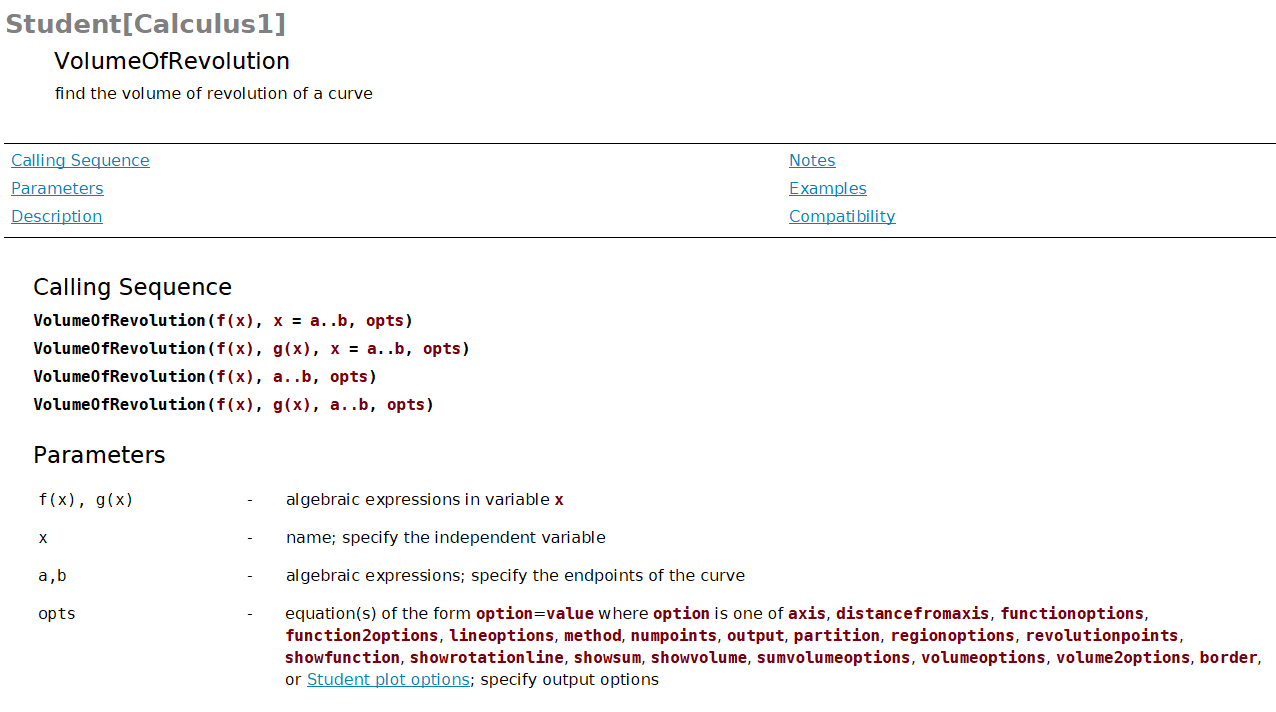
\includegraphics{figs/VolOfRev-help-page.png}

\BeginKnitrBlock{example}
\protect\hypertarget{exm:unnamed-chunk-91}{}{\label{exm:unnamed-chunk-91} }Show the solid obtained by rotating the region bounded by \(y=x^2\) and \(y=x\) about \(y\)-axis. Set up an integral for the volume. Find the volume.
\EndKnitrBlock{example}

\BeginKnitrBlock{solution}
\iffalse{} {Solution. } \fi{}

\#Load the package

\begin{verbatim}
with(Student[Calculus1])
\end{verbatim}

\#Show the solid

\begin{verbatim}
VolumeOfRevolution(x^2, x, x = 0 .. 1, axis = vertical, output = plot)
\end{verbatim}

\#Set up an integral

\begin{verbatim}
VolumeOfRevolution(x^2, x, x = 0 .. 1, axis = vertical, output = integral)
\end{verbatim}

\#Find the volume

\begin{verbatim}
VolumeOfRevolution(x^2, x, x = 0 .. 1, axis = vertical, output = value)
\end{verbatim}

The outputs in Maple can be seen in the following picture

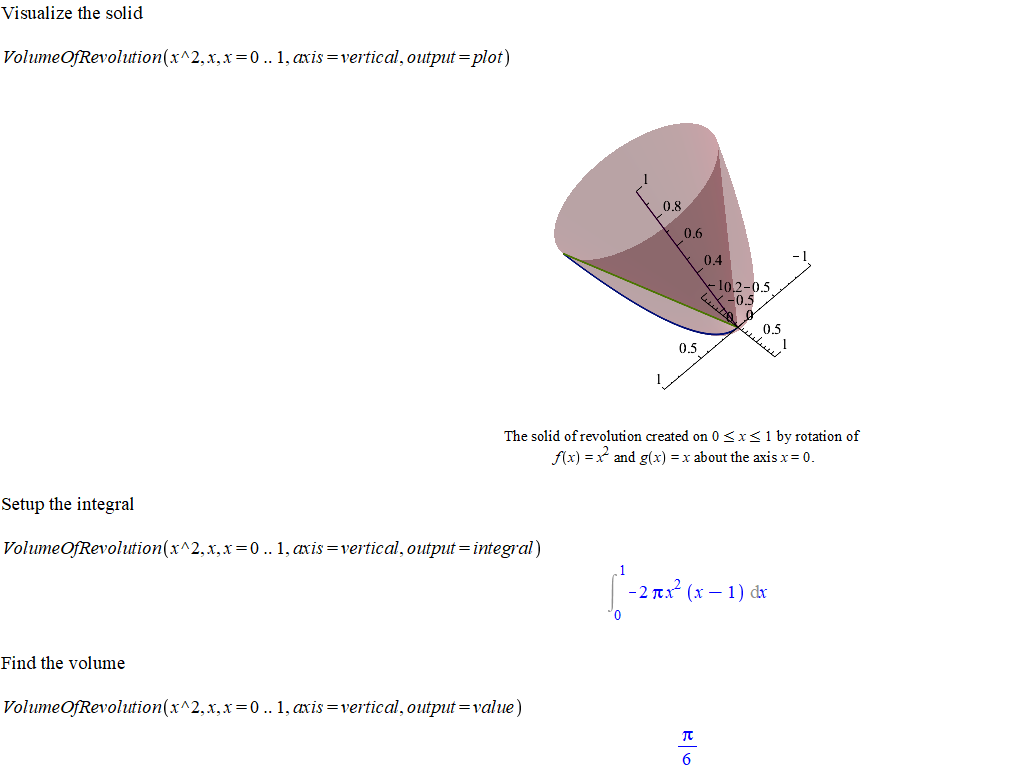
\includegraphics{figs/VolOfRev-Example1.png}
\EndKnitrBlock{solution}

\BeginKnitrBlock{remark}
\iffalse{} {Remark. } \fi{}1. If you change the function to \texttt{VolumeOfRevolutionTutor}, you will see an interactive popup windows which does exactly the same thing.

\begin{enumerate}
\def\labelenumi{\arabic{enumi}.}
\setcounter{enumi}{1}
\item
  If the rotation axis is not an axis of the coordinate system, you need add the option \texttt{distancefromaxis\ =\ numeric} into the function. For example, if in the above example, the rotation is about \(y=-2\), then the Maple command should be the following

\begin{verbatim}
 VolumeOfRevolution(x^2, x, x = 0 .. 1, axis = vertical, distancefromaxis = -2, output = integral)
\end{verbatim}
\end{enumerate}
\EndKnitrBlock{remark}

\BeginKnitrBlock{exercise}
\protect\hypertarget{exr:unnamed-chunk-94}{}{\label{exr:unnamed-chunk-94} }Find the volume of the solid obtained by rotating the region bounded by \(y=x^3\), \(x=0\), \(y=1\) about \(y\)-axis
\EndKnitrBlock{exercise}

\BeginKnitrBlock{exercise}
\protect\hypertarget{exr:unnamed-chunk-95}{}{\label{exr:unnamed-chunk-95} }Find the volume of the solid obtained by rotating the region bounded by \(y=x^3\), \(y=0\), \(x=1\) about (a) \(y=0\), and (b) \(x=2\).
\EndKnitrBlock{exercise}

\hypertarget{calculus-of-inverse-functions}{%
\chapter{Calculus of Inverse Functions}\label{calculus-of-inverse-functions}}

\hypertarget{inverse-functions}{%
\section{Inverse Functions}\label{inverse-functions}}

Maple package \texttt{Student{[}Calculus1{]}} provides the following command

\begin{verbatim}
InversePlot(f(x), x = a..b);
\end{verbatim}

which graphs the original function \(f(x)\) and the inverse function \(f^{-1}(x)\) together over the interval \([a, b]\).

You will see clearly that the graphs of a function and its inverse are symmetric with respect to the line \(y=x\).

\BeginKnitrBlock{example}
\protect\hypertarget{exm:unnamed-chunk-96}{}{\label{exm:unnamed-chunk-96} }

\begin{enumerate}
\def\labelenumi{\arabic{enumi}.}
\item
  Graph the function \(f(x)=x^3-2\), its inverse function, and the line \(y=x\) over the interval \([-2,2]\).
\item
  Find the inverse function.
\end{enumerate}
\EndKnitrBlock{example}

\BeginKnitrBlock{solution}
\iffalse{} {Solution. } \fi{}
One way to plot the function and its inverse together is to use the following command which is supported by the package \texttt{Student{[}Calculus1{]}}.

\begin{verbatim}
  InversePlot(x^3-3, x = -2 .. 2)
\end{verbatim}

Here is the output in Maple

\begin{figure}
\centering
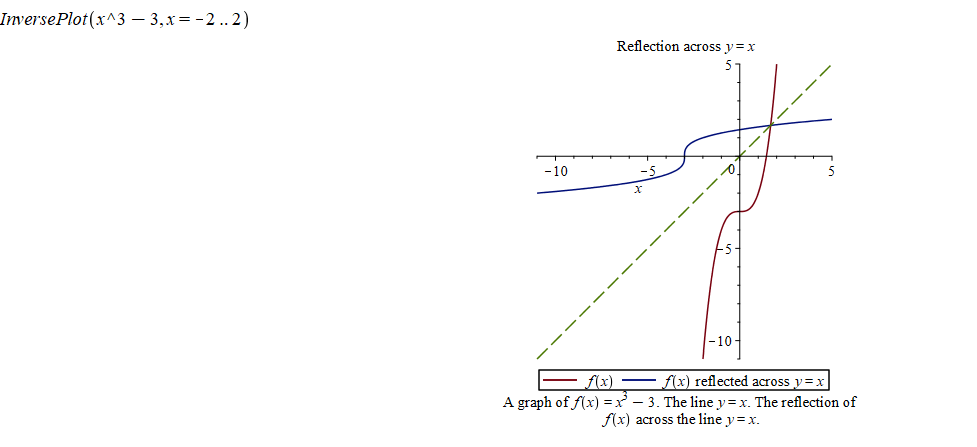
\includegraphics{figs/InversePlot1.png}
\caption{Graph of a pair of functions inverse to each other}
\end{figure}

Another way to plot the function \(f\) and its inverse \(g\) together uses the \texttt{plot} function.

\begin{verbatim}
  plot([f(x), g(x), x], x = -2 .. 4, y = -5 .. 5, color = [red, black, blue])
\end{verbatim}

To find the inverse function, we replace \(f(x)\) by \(y\), then switch \(x\) and \(y\), and solve for \(y\). In Maple, you may use the command \texttt{solve(equation/inequality,\ variable)} to solve an equation or an inequality (even system of equations/inequalities).

In this example, we may find the inverse function by type in the following command. Note I have switch \(x\) and \(y\).

\begin{verbatim}
solve(x=y^3, y)
\end{verbatim}
\EndKnitrBlock{solution}

To find the derivative of the inverse function of a function \(f\) at a given point \(x=a\), we may apply the formula
\[(f^{-1})'(a)=\dfrac{1}{f'(f^{-1}(a))}.\]
In Maple, we may use the following commands to calculate the value of the derivative function.

\begin{itemize}
\tightlist
\item
  Calculate the derivative of the function \(f\).
\end{itemize}

\begin{verbatim}

diff(f(x), x)
\end{verbatim}

\begin{itemize}
\tightlist
\item
  Find \(f^{-1}(a)\) which is the solution of the equaiton \(f(x)=a\).
\end{itemize}

\begin{verbatim}

solve(f(x)=a, x)
\end{verbatim}

\begin{itemize}
\tightlist
\item
  Plug in the formula to evaluate.
\end{itemize}

\begin{verbatim}

eval(subs(x=f^{-1}(a), 1/f'(x)))
\end{verbatim}

\BeginKnitrBlock{example}
\protect\hypertarget{exm:unnamed-chunk-98}{}{\label{exm:unnamed-chunk-98} }Find \((f^{-1})'(0)\), where \(f(x)=\cos(x)\) and \(0\leq x\leq \pi\).
\EndKnitrBlock{example}

\BeginKnitrBlock{solution}
\iffalse{} {Solution. } \fi{}
Find the derivative of \(f\)

\begin{verbatim}
diff(cos(x), x)
\end{verbatim}

Find the value of \(f^{-1}(0)\)

\begin{verbatim}
solve(cos(x)=0, x)
\end{verbatim}

Apply the formula

\begin{verbatim}
eval(subs(x=Pi/2, -1/sin(x)))
\end{verbatim}

Using Maple, we find \((f^{-1})'(0)=-1\).
\EndKnitrBlock{solution}

\BeginKnitrBlock{exercise}
\protect\hypertarget{exr:unnamed-chunk-100}{}{\label{exr:unnamed-chunk-100} }
1. Graph the function \(f(x)=3+2\sin x\), its inverse function, and the line \(y=x\) over the interval \([-2,2]\).

\begin{enumerate}
\def\labelenumi{\arabic{enumi}.}
\setcounter{enumi}{1}
\tightlist
\item
  Find the value \((f^{-1})'(5)\).
\end{enumerate}
\EndKnitrBlock{exercise}

\hypertarget{logarithmic-and-exponential-functions}{%
\section{Logarithmic and Exponential Functions}\label{logarithmic-and-exponential-functions}}

\hypertarget{basic-properties-and-graphs}{%
\subsection{Basic properties and graphs}\label{basic-properties-and-graphs}}

The natural logarithmic function \(y=\ln(x)\) is defined by \(\ln(x)=\int_1^x\frac{1}{t}\mathrm{d} t\).

The natural exponential function \(y=e^x\) is defined as the inverse function of \(y=\ln(x)\).

From the definition, we have very important identities
\[
\ln(e^x)=x\qquad \text{and}\qquad e^{\ln x}=x.
\]

Using those two identities, we may define general exponential functions and general logarithmic function, and deduce the Law of Logarithms and Law of Exponents.

\begin{itemize}
\item
  For any positive number \(b\ne 1\), we have \(b^x=(e^{\ln b})^x=e^{x\ln b}\).
\item
  For any positive number \(b\ne 1\), we define \(y=\log_bx\) to be the inverse function of \(y=b^x\)
\item
  By solving \(x=b^y\) for \(y\), we find that \(\log_bx=\dfrac{\ln x}{\ln b}\). This identity is called the change of base property.
\end{itemize}

How do graphs of logarithmic functions and exponential functions look like?

\BeginKnitrBlock{example}
\protect\hypertarget{exm:unnamed-chunk-101}{}{\label{exm:unnamed-chunk-101} }
Graph the following functions together.
\[
y=\ln x, \qquad y=e^x, \qquad y=2^x, \qquad y=\log_2x, y=x.
\]
\EndKnitrBlock{example}

\BeginKnitrBlock{solution}
\iffalse{} {Solution. } \fi{}
In Maple, the logarithm \(\log_bx\) is given by \texttt{log{[}b{]}(x)}. When \(b=e\), you simply use \texttt{ln(x)} for \(\ln x\). When \(b=10\), you may also use \texttt{log(x)} or \texttt{log10(x)} for \(\log_{10}x\).

The exponent \(b^x\) is given by \texttt{b\^{}x} in Maple. When \(b=e\), you may also use \texttt{exp(x)} to represent \(e^x\).

To graph the functions together with different colors, we use the following command

\begin{verbatim}
plot([ln(x), exp(x), 2^x, log[2](x), x], x=-5..5, color=[blue, green, purple, yellow, red])
\end{verbatim}

Here is the output

\begin{figure}
\centering
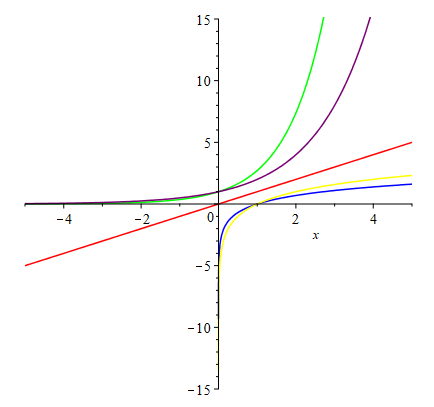
\includegraphics{figs/Log-Exp-Functions-01.png}
\caption{Graph of some logarithmic and exponential functions}
\end{figure}
\EndKnitrBlock{solution}

\BeginKnitrBlock{exercise}
\protect\hypertarget{exr:unnamed-chunk-103}{}{\label{exr:unnamed-chunk-103} }Graph the following functions together.
\[
y=\log_3x, \qquad y=3^x, \qquad y=(1/3)^x, \qquad y=\log_{1/3}x.
\]

Find the pairs that are symmetric to each other with respect to a certain line.
\EndKnitrBlock{exercise}

\BeginKnitrBlock{exercise}
\protect\hypertarget{exr:unnamed-chunk-104}{}{\label{exr:unnamed-chunk-104} }Graph the following functions together.
\[
y=0.5^x, \qquad y=2^x, \qquad y=5^x.
\]

Describe the monotonicity (increasing/decreasing) of the functions?

Fix an input \(x\). Describe how \(y\)-values change when bases changes from small number to bigger number?
\EndKnitrBlock{exercise}

\BeginKnitrBlock{exercise}
\protect\hypertarget{exr:unnamed-chunk-105}{}{\label{exr:unnamed-chunk-105} }Graph the following functions together.
\[
y=\log_{0.5}x, \qquad y=\log_2x, \qquad y=\log_{5}x.
\]

Describe the monotonicity (increasing/decreasing) of the functions?

Fix an input \(x\). Describe how \(y\)-values change when bases changes from small number to bigger number?
\EndKnitrBlock{exercise}

\hypertarget{differentiation-and-integration-of-logarithmic-and-exponential-functions}{%
\subsection{Differentiation and integration of logarithmic and exponential functions}\label{differentiation-and-integration-of-logarithmic-and-exponential-functions}}

In Maple, one way to do differentiation and integration is to use the \texttt{Calculus\ Palette} on the left side.

\begin{figure}
\centering
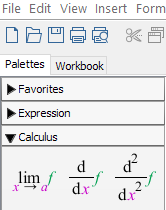
\includegraphics{figs/Calculus-Palette.png}
\caption{Calculus Palette in Maple}
\end{figure}

The other way is to use the commands \texttt{diff(f(x),\ x)} , \texttt{int(f(x),\ x)}, and \texttt{int(f(x),\ x=a..b)}.

Supported by the \texttt{Student{[}Calculus1{]}} package, Maple also provides the tutor commands \texttt{DiffTutor()} and \texttt{IntTutor()} which can show step-by-step solution of differentiation and integration.

Note you may also access tutor commands from the \texttt{Start} page (click the home button in the toolbar and look for Calculus).

\BeginKnitrBlock{example}
\protect\hypertarget{exm:unnamed-chunk-106}{}{\label{exm:unnamed-chunk-106} }Find \(y'\), where \(y=\ln \left(x^{3}+5x+1\right)\).
\EndKnitrBlock{example}

\BeginKnitrBlock{solution}
\iffalse{} {Solution. } \fi{}
Using \texttt{diff}:

\begin{verbatim}
diff(ln(x^3+5*x+1), x)
\end{verbatim}

We get
\[
y'=\dfrac{3x^{2}+5}{x^{3}+5 x+1}.
\]

Type in (assume that \texttt{with(Student{[}Calculus1{]})} was run)

\begin{verbatim}
DiffTutor(ln(x^3+5*x+1), x)
\end{verbatim}

and hit enter you will see

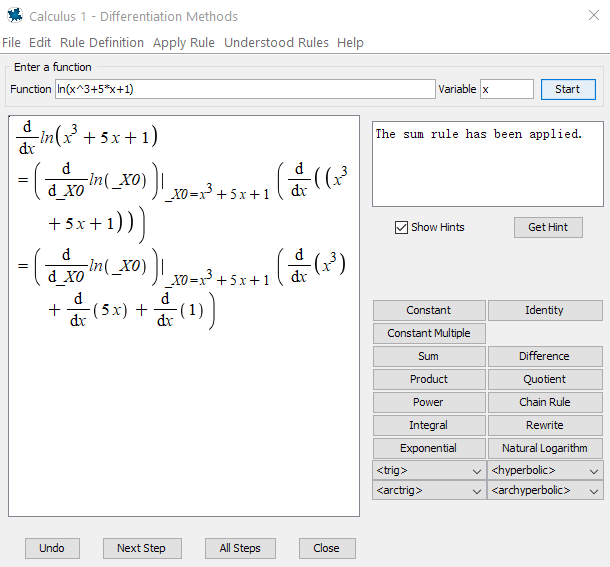
\includegraphics{figs/DiffTutor-ex.png}

By click \texttt{Next\ Step} or \texttt{All\ Steps} you will see detailed solution with rules used.
\EndKnitrBlock{solution}

\BeginKnitrBlock{example}
\protect\hypertarget{exm:unnamed-chunk-108}{}{\label{exm:unnamed-chunk-108} }Evaluate the integral
\[
\int\dfrac{e^x-1}{e^x+1}\mathrm{d} x.
\]
\EndKnitrBlock{example}

\BeginKnitrBlock{solution}
\iffalse{} {Solution. } \fi{}
Using \texttt{int}:

\begin{verbatim}
int((exp(x)-1)/(exp(x)+1), x)
\end{verbatim}

We get
\[
\int\dfrac{e^x-1}{e^x+1}\mathrm{d} x=2 \ln \left(\mathrm{e}^{x}+1\right)- x+C.
\]

Type in (assume that \texttt{with(Student{[}Calculus1{]})} was run)

\begin{verbatim}
IntTutor((exp(x)-1)/(exp(x)+1), x)
\end{verbatim}

and hit enter you will see

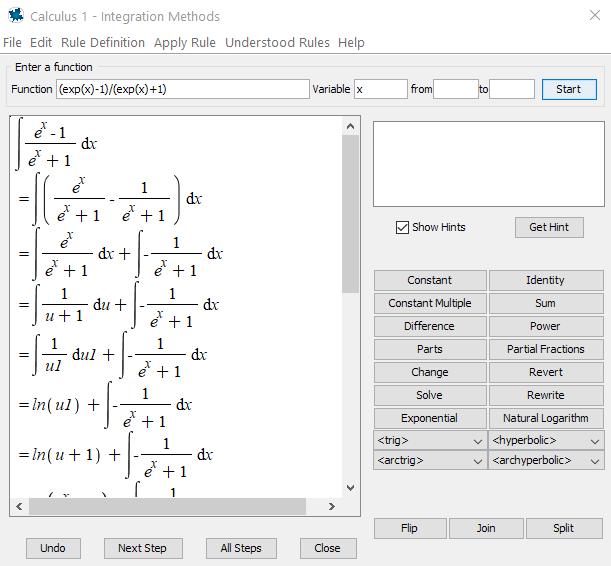
\includegraphics{figs/IntTutor-ex.png}

By click \texttt{Next\ Step} or \texttt{All\ Steps} you will see detailed solution with rules used.
\EndKnitrBlock{solution}

\BeginKnitrBlock{exercise}
\protect\hypertarget{exr:unnamed-chunk-110}{}{\label{exr:unnamed-chunk-110} }
Find the derivative \(\frac{\mathrm{d} y}{\mathrm{d} x}\), where \(y=\ln|\cos x|\)
\EndKnitrBlock{exercise}

\BeginKnitrBlock{exercise}
\protect\hypertarget{exr:unnamed-chunk-111}{}{\label{exr:unnamed-chunk-111} }
Find the derivative \(\frac{\mathrm{d} y}{\mathrm{d} x}\), where \(y=x^{\cos x}\)
\EndKnitrBlock{exercise}

\BeginKnitrBlock{exercise}
\protect\hypertarget{exr:unnamed-chunk-112}{}{\label{exr:unnamed-chunk-112} }
Evaluate the integral
\[
\int \frac{\left(e^{4x}+e^{2x}\right)}{e^{3x}} d x
\]
\EndKnitrBlock{exercise}

\BeginKnitrBlock{exercise}
\protect\hypertarget{exr:unnamed-chunk-113}{}{\label{exr:unnamed-chunk-113} }
Evaluate the integral
\[
\int 2^{3x} d x
\]
\EndKnitrBlock{exercise}

\hypertarget{solve-differential-equations}{%
\section{Solve differential equations}\label{solve-differential-equations}}

In Maple, you may solve the equation \(y'(x)=k y(x) + c\) (which is called an ODE) using the command \texttt{dsolve(\{ics,\ eq\})}, where \texttt{ics} stands for initial condition \(y(0)=c\) and \texttt{eq} stands for the differential equation. Without the \texttt{ics}, \texttt{dsolve} will provide a general solution.

\BeginKnitrBlock{example}
\protect\hypertarget{exm:unnamed-chunk-114}{}{\label{exm:unnamed-chunk-114} }Find the function \(f(x)\) which satisfies the differential equation \(f'(x)=k f(x)\) with \(f(0)=5\) and \(f(2)=3\).
\EndKnitrBlock{example}

\BeginKnitrBlock{solution}
\iffalse{} {Solution. } \fi{}
Use the following command

\begin{verbatim}
dsolve({f(0)=5, f'(x)=k f(x)})
\end{verbatim}

we get \(f(x)=5e^{kx}\).

To find \(k\), we solve the equation \(3=5e^{2k}\) by

\begin{verbatim}
solve(3=5*e^(2*k), k)
\end{verbatim}

which shows that \(k=\frac{\ln3-\ln5}{2}\approx -0.255\).
Here we use \texttt{evalf(\%)} (\% represents the previous result) to get the approximation.

So the function \(f\) is given by
\[
f(x)=5e^{\frac{x(\ln3-\ln5)}{2}}\approx 5e^{-0.255x}.
\]
\EndKnitrBlock{solution}

\BeginKnitrBlock{exercise}
\protect\hypertarget{exr:unnamed-chunk-116}{}{\label{exr:unnamed-chunk-116} }
Find the function \(y\) which satisfies the differential equation \(y'(x)=k y(x)\) with \(y(0)=2\) and \(y(5)=11\).
\EndKnitrBlock{exercise}

\hypertarget{inverse-trigonometric-functions}{%
\section{Inverse Trigonometric Functions}\label{inverse-trigonometric-functions}}

\hypertarget{domains-and-ranges}{%
\subsection{Domains and Ranges}\label{domains-and-ranges}}

To define the inverse function, the original function must be a one-to-one function.
For a trigonometric function, we have to restrict the function over a specific domain to ensure that the function is one-to-one.
For simplicity, we pick domains near the origin for trigonometric functions. To be more precise, we consider the following trigonometric functions:
\[
y=\sin x,\quad -\pi/2\leq x\leq \pi/2 ~~\text{and}~ -1\leq y\leq 1;
\]

\[
y=\cos x,\quad 0\leq x\leq \pi ~~\text{and}~ -1\leq y\leq 1;
\]

\[
y=\tan x,\quad -\pi/2< x< \pi/2 ~~\text{and}~ -\infty<y<\infty.
\]

Their inverse functions are

\[
y=\arcsin x,\quad -\pi/2\leq y\leq \pi/2 ~~\text{and}~ -1\leq x\leq 1;
\]

\[
y=\arccos x,\quad 0\leq y\leq \pi ~~\text{and}~ -1\leq x\leq 1;
\]

\[
y=\arctan x,\quad -\pi/2< y< \pi/2 ~~\text{and}~ -\infty< x<\infty.
\]

To see the graphs of the functions, we may use the \texttt{plot(f(x),\ x\ =\ a..b,\ opts)} command. Or, to graph \(f\), \(f^{-1}\) and \(y=x\) together, we may also use the command \texttt{InversePlot(f(x),\ x\ =\ a..b,\ opts)} supported by the package \texttt{Student{[}Calculus1{]}}.

\BeginKnitrBlock{example}
\protect\hypertarget{exm:unnamed-chunk-117}{}{\label{exm:unnamed-chunk-117} }
Graph the following functions together.
\[
y=\tan x, \qquad y=\arctan x, \qquad y=x.
\]
\EndKnitrBlock{example}

\BeginKnitrBlock{solution}
\iffalse{} {Solution. } \fi{}

\begin{verbatim}
#load the package ``Student[Calculus1]".
with(Student[Calculus1])
#plot the functions
InversePlot(tan(x),x=-Pi/2..Pi/2)
\end{verbatim}

Here is the output

\begin{figure}
\centering
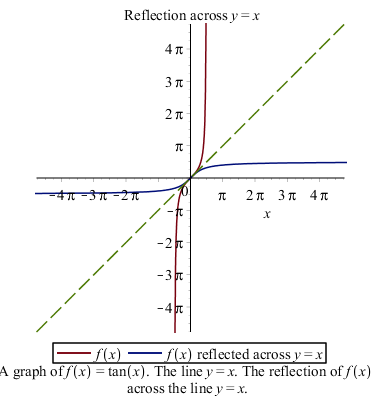
\includegraphics{figs/InversePlot_tanx.png}
\caption{Graph of the tangent and arctangent functions}
\end{figure}
\EndKnitrBlock{solution}

\BeginKnitrBlock{exercise}
\protect\hypertarget{exr:unnamed-chunk-119}{}{\label{exr:unnamed-chunk-119} }
Graph the following functions together over an appropriate domain.
\[
y=\cot x, \qquad y=\mathrm{arccot} x, \qquad y=x.
\]

What's the domain and range of \(y=\mathrm{arccot} x\)?
\EndKnitrBlock{exercise}

\hypertarget{differentiation-and-integration-of-inverse-trigonometric-functions}{%
\subsection{Differentiation and integration of inverse trigonometric functions}\label{differentiation-and-integration-of-inverse-trigonometric-functions}}

In the section \{\#Differentiation and integration of logarithmic and exponential functions\}, we learned to how use Maple to learn differentiation and integration.

Now let find derivatives and integrals of some inverse trigonometric functions.

\BeginKnitrBlock{example}
\protect\hypertarget{exm:unnamed-chunk-120}{}{\label{exm:unnamed-chunk-120} }
Find \(y'\), where \(y=\mathrm{arccot} x\).
\EndKnitrBlock{example}

\BeginKnitrBlock{solution}
\iffalse{} {Solution. } \fi{}

Surely, we may use \texttt{diff} or \texttt{DiffTutor} to find the derivative.

Here let's me introduce to you another command \texttt{implicitdiff}.

We've learned that (see \{\#Inverse Functions\}) to find the inverse function, we switch \(x\) and \(y\) and then solve for \(y\). When finding the derivative, we don't have to solve for \(y\) instead, we want \(y'\) which is implicitly defined by an equation. In this case, we have \(x=\mathrm{arccot}y\).

Enter the following commands in Maple, you will find \(y'=-\frac{1}{x^2+1}\).

\begin{verbatim}
implicitdiff(x=cot(y), y, x)
subs(cot(y) = x, %)
\end{verbatim}

where \texttt{\%} is a ditto operator that allows you to refer to a previously computed result in Maple.
\EndKnitrBlock{solution}

\BeginKnitrBlock{exercise}
\protect\hypertarget{exr:unnamed-chunk-122}{}{\label{exr:unnamed-chunk-122} }
Find the derivative of \(y=\mathrm{arcsec} x\)
\EndKnitrBlock{exercise}

\BeginKnitrBlock{exercise}
\protect\hypertarget{exr:unnamed-chunk-123}{}{\label{exr:unnamed-chunk-123} }
Find the derivative of \(y=\mathrm{arccsc} x\)
\EndKnitrBlock{exercise}

For integrals of inverse trigonometric function, you may need the method of integration by parts.

Use \texttt{DiffTutor} to find antiderivatives of inverse trigonometric functions.

\BeginKnitrBlock{exercise}
\protect\hypertarget{exr:unnamed-chunk-124}{}{\label{exr:unnamed-chunk-124} }
Evaluate the integral
\[
\int \arcsin x \mathrm{d} x
\]
\EndKnitrBlock{exercise}

\BeginKnitrBlock{exercise}
\protect\hypertarget{exr:unnamed-chunk-125}{}{\label{exr:unnamed-chunk-125} }
Evaluate the integral
\[
\int \arctan x \mathrm{d} x
\]
\EndKnitrBlock{exercise}

\BeginKnitrBlock{exercise}
\protect\hypertarget{exr:unnamed-chunk-126}{}{\label{exr:unnamed-chunk-126} }
Evaluate the integral
\[
\int \mathrm{sec} x \mathrm{d} x
\]
\EndKnitrBlock{exercise}

\hypertarget{lhospitals-rule}{%
\section{L'Hospital's Rule}\label{lhospitals-rule}}

In Maple, supported by the package, \texttt{Student{[}Calculus1{]}}, the command \texttt{LimitTutor} can show step-by-step solutions of evaluating limits.

\BeginKnitrBlock{example}
\protect\hypertarget{exm:unnamed-chunk-127}{}{\label{exm:unnamed-chunk-127} }
Evaluate the limit
\[
\lim\limits_{x\to \infty}(1+x)^{1/\ln(x)}
\]
\EndKnitrBlock{example}

\BeginKnitrBlock{solution}
\iffalse{} {Solution. } \fi{}

\begin{verbatim}
# load the package Student[Calculus1].
with(Student[Calculus1])
#Find the limit step-by-step using LimitTutor
LimitTutor((1+x)^(1/ln(x)), x = infinity)
\end{verbatim}
\EndKnitrBlock{solution}

\BeginKnitrBlock{exercise}
\protect\hypertarget{exr:unnamed-chunk-129}{}{\label{exr:unnamed-chunk-129} }
Estimate the limit
\[
\lim\limits_{x\to 1}\frac{x^2-2x+1}{x^2-x}
\]
by graphing and verify your estimation.
\EndKnitrBlock{exercise}

\BeginKnitrBlock{exercise}
\protect\hypertarget{exr:unnamed-chunk-130}{}{\label{exr:unnamed-chunk-130} }
Evaluate the limit
\[
\lim\limits_{x\to \infty} x-\ln(x).
\]
\EndKnitrBlock{exercise}

\BeginKnitrBlock{exercise}
\protect\hypertarget{exr:unnamed-chunk-131}{}{\label{exr:unnamed-chunk-131} }
Evaluate the limit
\[
\lim\limits_{x\to \infty} x\tan(\frac1x).
\]
\EndKnitrBlock{exercise}

\hypertarget{techniques-of-integration}{%
\chapter{Techniques of Integration}\label{techniques-of-integration}}

\hypertarget{integrations-of-trigonometric-functions}{%
\section{Integrations of trigonometric functions}\label{integrations-of-trigonometric-functions}}

When evaluating integrations of trigonometric functions, one idea is to reduce the total degree (power) of trigonometric functions using trigonometric identities.

In Maple, you may use the command \texttt{combine} to rewrite the expression.

\BeginKnitrBlock{example}
\protect\hypertarget{exm:unnamed-chunk-132}{}{\label{exm:unnamed-chunk-132} }
Rewrite \(\cos^4x\) into an expression with single terms and evaluate the integral \(\int \cos^4x\mathrm{d} x\).
\EndKnitrBlock{example}

\BeginKnitrBlock{solution}
\iffalse{} {Solution. } \fi{}

\begin{verbatim}
# combine terms into a single term
combine((cos(x))^4)
# use DiffTutor to evaluate the integral of the resulting function.
with(Student[Calculus1])
IntTutor(%, x)
\end{verbatim}
\EndKnitrBlock{solution}

You may compare the above solution with the solution given by \texttt{IntTutor((cos(x))\^{}4,\ x)}.

\BeginKnitrBlock{exercise}
\protect\hypertarget{exr:unnamed-chunk-134}{}{\label{exr:unnamed-chunk-134} }
Evaluate the integral
\[
\int \tan ^{5} x \mathrm{d} x
\]
\EndKnitrBlock{exercise}

\BeginKnitrBlock{exercise}
\protect\hypertarget{exr:unnamed-chunk-135}{}{\label{exr:unnamed-chunk-135} }
Evaluate the integral
\[
\int \sin 5 x \sin^2 x \mathrm{d} x
\]
\EndKnitrBlock{exercise}

\hypertarget{trigonometric-substitution}{%
\section{Trigonometric Substitution}\label{trigonometric-substitution}}

Surely, you may learn some trigonometric substitution tricks using \texttt{IntTutor}.

Here I want to introduce another useful command which when integrating functions, we may need to complete a square and then do a substitution. In Maple, we can complete squares using the command \texttt{CompleteSquare(f,\ x)} which supported by the package \texttt{Student{[}Precalculus{]}}.

\BeginKnitrBlock{example}
\protect\hypertarget{exm:unnamed-chunk-136}{}{\label{exm:unnamed-chunk-136} }
Evaluate the integral
\[
\int\dfrac{1}{x^2+x+1} \mathrm{d} x.
\]
\EndKnitrBlock{example}

\BeginKnitrBlock{solution}
\iffalse{} {Solution. } \fi{}

We first complete the square for the denominator.

\begin{verbatim}
#load package Student[Precalculus]
with(Student[Precalculus])
#Complete square for the denominator
CompleteSquare(x^2+x+1, x)
\end{verbatim}

Now you may try \texttt{DiffTutor} and/or evaluate it by hand.

\begin{verbatim}
#load package Student[Calculus1]
with(Student[Calculus1])
DiffTutor(1/%, x)
\end{verbatim}
\EndKnitrBlock{solution}

\BeginKnitrBlock{exercise}
\protect\hypertarget{exr:unnamed-chunk-138}{}{\label{exr:unnamed-chunk-138} }
Evaluate the integral
\[
\int \sqrt{3+2 x-x^{2}} \mathrm{d} x
\]
\EndKnitrBlock{exercise}

\BeginKnitrBlock{exercise}
\protect\hypertarget{exr:unnamed-chunk-139}{}{\label{exr:unnamed-chunk-139} }
Evaluate the integral
\[
\int_{0}^{\pi / 2} \frac{\cos t}{\sqrt{1+\sin ^{2} t}} \mathrm{d} t
\]
\EndKnitrBlock{exercise}

\hypertarget{integrations-of-rational-functions-by-partial-fractions}{%
\section{Integrations of Rational Functions by Partial Fractions}\label{integrations-of-rational-functions-by-partial-fractions}}

In Maple, we can factor a polynomial using the command \texttt{factor(polynomial)} or find partial fraction decomposition using \texttt{convert(function,\ parfrac)}.

\BeginKnitrBlock{example}
\protect\hypertarget{exm:unnamed-chunk-140}{}{\label{exm:unnamed-chunk-140} }
Find the sum of partial fractions for the rational function
\[
f(x)=\frac{x^3+4x+3}{x^4+5x^2+4}
\]
\EndKnitrBlock{example}

\BeginKnitrBlock{solution}
\iffalse{} {Solution. } \fi{}
This can be done easily in Maple:

\begin{verbatim}
# use the command convert
convert((x^3+4*x+3)/(x^4+5x^2+4), parfrac)
\end{verbatim}
\EndKnitrBlock{solution}

\BeginKnitrBlock{exercise}
\protect\hypertarget{exr:unnamed-chunk-142}{}{\label{exr:unnamed-chunk-142} }
Find the sum of partial fractions for the rational function
\[
f(x)=\frac{x^{4}}{\left(x^{2}-x+1\right)\left(x^{2}+2\right)^{2}}.
\]
\EndKnitrBlock{exercise}

\BeginKnitrBlock{exercise}
\protect\hypertarget{exr:unnamed-chunk-143}{}{\label{exr:unnamed-chunk-143} }
Find the sum of partial fraction and evaluate the integral

\[
\int \frac{2}{3x^{2}+2x-1} \mathrm{d} x
\]
\EndKnitrBlock{exercise}

\BeginKnitrBlock{exercise}
\protect\hypertarget{exr:unnamed-chunk-144}{}{\label{exr:unnamed-chunk-144} }
Find the sum of partial fraction and evaluate the integral

\[
\int \frac{x^{3}+6 x-2}{x^{4}+6 x^{2}} \mathrm{d} x
\]
\EndKnitrBlock{exercise}

\BeginKnitrBlock{exercise}
\protect\hypertarget{exr:unnamed-chunk-145}{}{\label{exr:unnamed-chunk-145} }
Find the sum of partial fraction and evaluate the integral

\[
\int \frac{\sin x}{\cos ^{2} x-3 \cos x} d x
\]
\EndKnitrBlock{exercise}

\hypertarget{further-applications-of-integration}{%
\chapter{Further Applications of Integration}\label{further-applications-of-integration}}

\hypertarget{arc-lengths-and-areas-of-surfaces-of-revolutions}{%
\section{Arc Lengths and Areas of Surfaces of Revolutions}\label{arc-lengths-and-areas-of-surfaces-of-revolutions}}

\begin{itemize}
\item
  \textbf{Arc length:}

  The length \(L\) of an arc: \(y=f(x)\), \(a\leq x \leq b\) is
  \[
  L=\int_a^b\sqrt{1+\left(\frac{\mathrm{d} y}{\mathrm{d} x}\right)^2}~\mathrm{d} x=\int_{f(a)}^{f(b)}\sqrt{1+\left(\frac{\mathrm{d} y}{\mathrm{d} x}\right)^2}~\mathrm{d} y.
  \]
\item
  \textbf{Surface area of a revolution}

  The area \(S\) of the surface rotating an arc: \(y=f(x)\), \(a\leq x \leq b\) about the \(x\)-axis is
  \[
  S=2\pi\int r\mathrm{d} s = 2\pi\int y\mathrm{d} s,
  \]
  and about the \(y\)-axis is
  \[
  S=2\pi\int r\mathrm{d} s = 2\pi\int x\mathrm{d} s,
  \]
  where
  \[\mathrm{d} s=\sqrt{1+\left(\frac{\mathrm{d} y}{\mathrm{d} x}\right)^2}~\mathrm{d} x = \sqrt{1+\left(\frac{\mathrm{d} y}{\mathrm{d} x}\right)^2}~\mathrm{d} y.
  \]
  The integral limits depend on whether you use \(\mathrm{d} x\) or \(\mathrm{d}y\) in the integral.
\end{itemize}

In Maple, the package \texttt{Student{[}Calculus1{]}} provides commands to investigate arc length and surface area of revolutions:
\texttt{ArcLength(f(x),\ x\ =\ a..b,\ opts)\}}
\texttt{SurfaceOfRevolution(f(x),\ x\ =\ a..b,\ opts)\}}

\BeginKnitrBlock{example}
\protect\hypertarget{exm:unnamed-chunk-146}{}{\label{exm:unnamed-chunk-146} }
Set up an integral and evaluate the integral for the length of the curve defined by
\[
f(x)=\sqrt{x},\qquad 1\leq x\leq 4.
\]
Plot \(f(x)\) together with the arc length function in the same coordinate system.
\EndKnitrBlock{example}

\BeginKnitrBlock{solution}
\iffalse{} {Solution. } \fi{}

\begin{verbatim}
# Load the package

with(Student[Calculus1])

# Set up an integral

ArcLength(sqrt(x),x=1..4,output=integral)

# Evaluate the integral

ArcLength(sqrt(x),x=1..4)

# Plot the function and the arc length function

ArcLength(sqrt(x), x=1..4, output=plot)
\end{verbatim}
\EndKnitrBlock{solution}

\BeginKnitrBlock{example}
\protect\hypertarget{exm:unnamed-chunk-148}{}{\label{exm:unnamed-chunk-148} }
Set up an integral and evaluate the integral for the area of the surface obtained by rotating the curve defined by
\[
f(x)=\sqrt{x},\qquad 1\leq x\leq 4
\]
about the \(y\)-axis. Plot the surface of the revolution.
\EndKnitrBlock{example}

\BeginKnitrBlock{solution}
\iffalse{} {Solution. } \fi{}

\begin{verbatim}
# Load the package (skip if the package was already loaded)

with(Student[Calculus1])

# Plot the surface

SurfaceOfRevolution(sqrt(x), x=1..4, output=plot, axis=vertical)

# Set up an integral

SurfaceOfRevolution(sqrt(x),x=1..4,output=integral, axis=vertical)

# Evaluate the integral

SurfaceOfRevolution(sqrt(x),x=1..4, axis=vertical)
\end{verbatim}
\EndKnitrBlock{solution}

\BeginKnitrBlock{exercise}
\protect\hypertarget{exr:unnamed-chunk-150}{}{\label{exr:unnamed-chunk-150} }
Set up an integral and evaluate the integral for the length of the arc defined by
\[
f(x)=\ln x, \qquad 1\leq x\leq 2.
\]
Plot \(f(x)\) together with the arc length function in the same coordinate system.
\EndKnitrBlock{exercise}

\BeginKnitrBlock{exercise}
\protect\hypertarget{exr:unnamed-chunk-151}{}{\label{exr:unnamed-chunk-151} }
Plot the surface obtained by rotating the curve defined by
\[
f(x)=\frac{\cos x}{x}, \qquad 0\leq x\leq 4\pi
\]
about the \(y\)-axis. Set up an integral for the area of the surface.
\EndKnitrBlock{exercise}

\BeginKnitrBlock{exercise}
\protect\hypertarget{exr:unnamed-chunk-152}{}{\label{exr:unnamed-chunk-152} }
Find the area of the surface obtained by rotating the curve defined by
\[
f(x)=\sqrt{1+x^2},\qquad 0\leq x\leq 3.
\]
\EndKnitrBlock{exercise}

\hypertarget{infinite-sequences-and-series}{%
\chapter{Infinite Sequences and Series}\label{infinite-sequences-and-series}}

\hypertarget{introduction-to-sequences-and-series}{%
\section{Introduction to Sequences and Series}\label{introduction-to-sequences-and-series}}

A sequence is a list of numbers in a definite order (indexed by integers). A series may be considered as the limit of the sequence of partial sums.

When the sequence is explicitly defined by an mathematical expression \(a_n=f(n)\), Maple has the following command to list numbers of the sequence \texttt{seq(f,\ i=m..n,\ step)}.

\BeginKnitrBlock{example}
\protect\hypertarget{exm:seq-eg}{}{\label{exm:seq-eg} }
Find the first 10 terms of the sequence \(\{\frac{1}{n(n+1)}\}_{n=1}^\infty\). Determine whether the sequence \(\{\frac{1}{n(n+1)}\}\) is convergent or divergent.
\EndKnitrBlock{example}

\BeginKnitrBlock{solution}
\iffalse{} {Solution. } \fi{}

\begin{verbatim}
# using seq

seq(1/(n*(n+1)), n=1..10)
\end{verbatim}

The sequence converges to \(0\).
\EndKnitrBlock{solution}

For a series \(\sum a_n\), normally it is not easy to find explicit expression for the partial sum \(s_n=\sum\limits_{k=1}^n a_k\). However, if sequence is defined by an mathematical expression \(a_n=f(n)\), we may find values of partial sums recursively use a \texttt{for/from\ loop} statement in Maple:

\begin{verbatim}
for *counter* from *initial* by *increment* to *final* do
    statement_sequence;
end do;
\end{verbatim}

\BeginKnitrBlock{example}
\protect\hypertarget{exm:unnamed-chunk-154}{}{\label{exm:unnamed-chunk-154} }
Find the first 20 partial sums \(s_k=\sum_{n=1}^{n}a_n\) of the infinite series
\[
\sum_{n=0}^\infty\frac1{2^n}=1+\frac12+\frac14+\frac18+\cdots.
\]
Determine whether the series \(\sum_{n=0}^\infty\frac1{2^n}\) is convergent or divergent.
\EndKnitrBlock{example}

\BeginKnitrBlock{solution}
\iffalse{} {Solution. } \fi{}

\begin{verbatim}
# Set up s when n=0

s:=1

# Find 10 terms using `for/from loop`

for n from 1 to 10 do
    s:=s+1/(2^n);
end do;
\end{verbatim}

The series converges to 2.
\EndKnitrBlock{solution}

Of course, we may also use \texttt{for/from\ loop} to list numbers of a sequence.

\BeginKnitrBlock{solution}
\iffalse{} {Solution. } \fi{}Second solution to example \ref{exm:seq-eg}.

\begin{verbatim}
# using `for/from loop`

for n from 1 to 10 do
    1/(n*(n+1);
end do;
\end{verbatim}
\EndKnitrBlock{solution}

When the sequence is defined by a recurrence formula like the Fibonacci sequence, we will need to Maple how to interpret the formula. For that purpose, we use a procedure, which encloses a sequence of statements between \texttt{proc(...)} and \texttt{end\ proc}, to define the formula in Maple.

For example, the following is a procedure that defines a function \(a(x)=\sqrt{x}-\frac{1}{\sqrt{x}}\):

\begin{verbatim}
a:=proc(x) sqrt(x)-1/sqrt{x}; end proc;
\end{verbatim}

To structure codes in a procedure, you may use \texttt{Code\ Edit\ Region} which can be find in the \texttt{Insert\ menu}.
To execute codes within this region, click \texttt{Execute\ Code} from the \texttt{Edit} menu, or use the shortcut command \texttt{Ctrl+E}.

\BeginKnitrBlock{example}
\protect\hypertarget{exm:unnamed-chunk-157}{}{\label{exm:unnamed-chunk-157} }
The Fibonacci sequence is defined by \(fib(0)=0\), \(fib(1)=1\) and \(fib(n)=fib(n-1)+fic(n-2)\).
Find the first 20 Fibonacci numbers.
\EndKnitrBlock{example}

\BeginKnitrBlock{solution}
\iffalse{} {Solution. } \fi{}
We first define a function \(fib(n)\) which returns the \(n\)-th Fibonacci number.

\begin{verbatim}
fib := proc (n::nonnegint)
    if 2 <= n then
        return fib(n-1)+fib(n-2):
    else
        return n:
    end if;
end proc
\end{verbatim}

Now we can use either \texttt{seq()} or \texttt{for/from\ loop}.

seq(fib(n), n=0..19)
\EndKnitrBlock{solution}

\BeginKnitrBlock{exercise}
\protect\hypertarget{exr:unnamed-chunk-159}{}{\label{exr:unnamed-chunk-159} }
Find the first 20 terms of the sequence
\[
\{\sin{\frac{\pi}{n}}\}_{n=1}^\infty.
\]
Determine whether the sequence \(\{\sin{\frac{\pi}{n}}\}\) is convergent or divergent.
\EndKnitrBlock{exercise}

\BeginKnitrBlock{exercise}
\protect\hypertarget{exr:unnamed-chunk-160}{}{\label{exr:unnamed-chunk-160} }
Find the first 20 partial sums \(s_k=\sum_{n=1}^{n}a_n\) of the infinite series
\[\sum_{n=0}^\infty\frac1n=1+\frac12+\frac13+\frac14+\cdots.
\]
Determine whether the series \(\sum_{n=0}^\infty\frac1n\) is convergent or divergent.
\EndKnitrBlock{exercise}

\BeginKnitrBlock{exercise}
\protect\hypertarget{exr:unnamed-chunk-161}{}{\label{exr:unnamed-chunk-161} }
Find the 20th to 30th Fibonacci numbers.
\EndKnitrBlock{exercise}

\hypertarget{power-series}{%
\section{Power Series}\label{power-series}}

A power series is a series with a variable \(x\):
\[
\sum\limits_{n=0}^{\infty} c_nx^n=c_0+c_1x+c_2x^2+c_3x^3+\cdots.
\]

More generally, a series of the form

\begin{equation}
\sum\limits_{n=0}^{\infty} c_n(x-a)^n=c_0+c_1(x-a)+c_2(x-a)^2+c_3(x-a)^3+\cdots
\label{eq:Taylor-series}
\end{equation}

is called a power series at \(a\).

We call a positive number \(R\) the radius of convergence of the power series \ref@(eq:Taylor-series) if the power series converges whenever \(\left|x-a\right|<R\) and diverges whenever \(\left|x-a\right|>R\).

If a function \(f\) has a power series representation, i.e.
\[
f(x)=\sum_{n=0}^\infty c_n(x-a)^n,\quad\quad \left|x-a\right|<R,
\]
then its coefficients are given by \(c_n=\dfrac{f^{(n)}(a)}{n!}.\)

\BeginKnitrBlock{example}
\protect\hypertarget{exm:unnamed-chunk-162}{}{\label{exm:unnamed-chunk-162} }
Find the interval of convergence of the power series
\[
\sum\limits_{n=1}^{\infty}\dfrac{(-2)^nx^n}{n^3}.
\]
\EndKnitrBlock{example}

\BeginKnitrBlock{solution}
\iffalse{} {Solution. } \fi{}

\begin{verbatim}
# Find the abs(a_{n+1}/a_n)

q:=abs((-2)^(n+1)(n+1)^3/(-2)^(n+1)(n+1)^3);

# Find the limit of q

r:=limit(simplify(q), n=infinity)

# Find the interval of convergence

solve(abs(x)<1/r, x)
\end{verbatim}
\EndKnitrBlock{solution}

\BeginKnitrBlock{example}
\protect\hypertarget{exm:unnamed-chunk-164}{}{\label{exm:unnamed-chunk-164} }
Find the Taylor expansion of the function \(f(x)=\dfrac{1}{x-2}\) at \(x=0\) up to the 5-th order. Plot \(f(x)\) and the \(5\)-th order Taylor polynomial together.
\EndKnitrBlock{example}

\BeginKnitrBlock{solution}
\iffalse{} {Solution. } \fi{}

\begin{verbatim}
# Find the Taylor expansion.

ftaylor:=taylor(1/(x-2), x = 0, 5)

# convert the Taylor series into a polynomial

fpoly:=convert(ftaylor, polynom)

# Plot the functions

plot([1/(x-2), fpoly], x=-1..1)
\end{verbatim}
\EndKnitrBlock{solution}

\BeginKnitrBlock{exercise}
\protect\hypertarget{exr:unnamed-chunk-166}{}{\label{exr:unnamed-chunk-166} }
Find the interval of convergence of the power series
\[
\sum\limits_{n=1}^{\infty}\dfrac{(-4)^nx^n}{\sqrt{n}}.
\]
\EndKnitrBlock{exercise}

\BeginKnitrBlock{exercise}
\protect\hypertarget{exr:unnamed-chunk-167}{}{\label{exr:unnamed-chunk-167} }
Find the Taylor expansion of the function \(f(x)=\sin x\) at \(x=0\) up to the 5-th order. Plot \(f(x)\) and the \(5\)-th order Taylor polynomial together over the interval \([-\pi,\pi]\).
\EndKnitrBlock{exercise}

\hypertarget{taylor-expansion}{%
\section{Taylor Expansion}\label{taylor-expansion}}

Let \(f(x)\) be a function. Assume that the \(k\)-th order derivatives \(f^k(a)\) exist for \(k=1, 2, \dots, n\). The polynomial
\[
T_n(x)=\sum_{k=0}^n\dfrac{f^{(n)}(a)}{k!}(x-a)^k
\]
is called the \(n\)-th degree Taylor polynomial of \(f\) at \(a\).

Let \(f(x)\) be a function has derivative at \(a\) up to all orders. Set
\[
R_n(x)=\sum_{k=n+1}^\infty \dfrac{f^{(k)}(a)}{k!}(x-a)^k,\quad\quad \left|x-a\right|<R,
\]
which is called the reminder of the Taylor series
\[
\sum\limits_{k=0}^\infty \dfrac{f^{(k)}(a)}{k!}(x-a)^k.
\]

If
\[
\lim\limits_{n\to\infty} R_n(x)=0
\]
for \(\left|x-a\right|<R\), then \(f(x)\) is the sum of the Taylor series on the interval, that is
\[
f(x)=\sum\limits_{k=0}^\infty \dfrac{f^{(k)}(a)}{k!}(x-a)^k,\quad\quad \left|x-a\right|<R.
\]

If \(\left|f^{n+1}{x}\right|\leq M\) for \(\left|x-a\right|\leq d\), then the reminder \(R_n\) satisfies the follow inequality
\[
\left|R_n(x)\right|\leq \dfrac{M}{n+1}\left|x-a\right|^{n+1}\quad \text{for}\quad \left|x-a\right|\leq d.
\]

Roughly speaking, the absolute value of the reminder \(\left|R_n(x)\right|\) determines how accurate the Taylor polynomial approximation.

\BeginKnitrBlock{example}
\protect\hypertarget{exm:unnamed-chunk-168}{}{\label{exm:unnamed-chunk-168} }
Approximate function \(f(x)=\sin x\) by the degree 3 Taylor polynomial at \(x=1\).
\EndKnitrBlock{example}

\BeginKnitrBlock{solution}
\iffalse{} {Solution. } \fi{}

\begin{verbatim}
# Find the Taylor series.

fTs:=taylor(sin(x), x = 0, 4)

# Convert the Taylor series into a polynomial

fTp:=convert(fTs, polynom)

# Evaluate the Taylor polynomial at 1

subs(x=1, fpolyapprox)
\end{verbatim}
\EndKnitrBlock{solution}

\BeginKnitrBlock{example}
\protect\hypertarget{exm:unnamed-chunk-170}{}{\label{exm:unnamed-chunk-170} }
Plot the function
\[
g(x)=\begin{cases}e^{-\frac{1}{x^2}} & x\neq 0\\ 0 & x=0\end{cases}
\]
and its 5-th order Taylor polynomial over the domain \([-2..2]\). What can you conclude?
\EndKnitrBlock{example}

\BeginKnitrBlock{solution}
\iffalse{} {Solution. } \fi{}

\begin{verbatim}
# Define a piece-wisely defined function.

g:=piecewise(x!=0, exp(-1/x^2), 0)

# Find Taylor polynomial of degree 5.

for n to 5 do T := (eval(diff(g(x), x$n), x = 0))*x^n/factorial(n)+T end do

# Plot the functions

plot([g,T],x=-2..2, color=[red, blue])
\end{verbatim}

The graphs of the functions are shown in the picture.
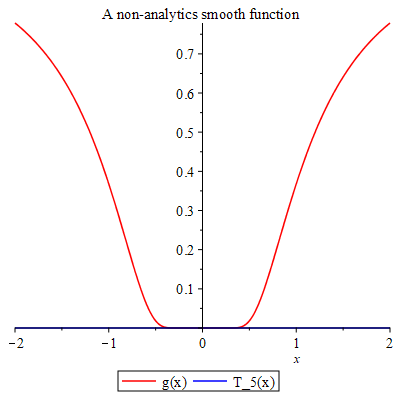
\includegraphics{figs/non-analytic-smooth.png}
\EndKnitrBlock{solution}

In the solution, \texttt{x\$n} is a shortcut option for \texttt{x,\ x,\ x,\ x,\ x} in the \texttt{diff} command.

\BeginKnitrBlock{exercise}
\protect\hypertarget{exr:unnamed-chunk-172}{}{\label{exr:unnamed-chunk-172} }
Approximate function \(f(x)=e^x\) by the degree 5 Taylor polynomial at \(x=1\).
\EndKnitrBlock{exercise}

\BeginKnitrBlock{exercise}
\protect\hypertarget{exr:unnamed-chunk-173}{}{\label{exr:unnamed-chunk-173} }
Compare the function \(y=\sin x\) with its degree 10 Taylor polynomial at \(x=0\).
\EndKnitrBlock{exercise}


\end{document}
